\chapter{
 Closed Population Models
}
\markboth{Chapter 3}{}
\label{chapt.closed}

\vspace{.3in}

Having covered some basics of standard % "standard" is a little vague
models and their implementation in \textbf{BUGS} software,
in this chapter we will consider ordinary capture-recapture (CR)
models for estimating population size in closed populations. A closed
population is one whose abundance $N$ does not change during the
study. Two forms of closure are often discussed: demographic closure,
meaning that no births or deaths occur, and geographic closure, which
states that no individuals move onto or off of the plot during the study.
Few populations are actually closed except during very short
time intervals, but closed population CR models serve as the basis for
the development of the rest of the models presented in this book,
including the models for open populations discussed in
Chapt.\ref{chapt.open}.

We will
see that classical closed population CR models are closely related to binomial (or logistic)
regression-type models. In fact, when $N$ is known, they are precisely
logistic regression models.  We consider some important extensions of ordinary closed
population models that accommodate various types of ``individual
effects'' --- either in the form of explicit, observed %and measured
covariates (sex, age,
body mass) or unstructured ``heterogeneity'' in the form of an
individual random effect, which represent effects of unobserved or
unmeasured covariates. In general, these models are variations of
generalized linear or generalized linear mixed models (GLMs and GLMMs, respectively).
Because of the paramount importance of this concept, we focus mainly
on fairly simple models in which the observations are individual
encounter frequencies, $y_{i}$ = the number of encounters of
individual $i$ out of $K$ replicate samples of the population which,
for the models we consider here, is the outcome of a binomial random
variable.  Along the way, we consider the spatial context of
capture-recapture data %and models
and demonstrate that density cannot
be formally estimated when spatial information is ignored. We also
review some of the informal methods of estimating density using CR
methods, and consider some of their limitations.  We will be exposed
to our first primitive spatial capture-recapture models which arise as
relatively minor variations of so-called ``individual covariate
models'' (of the \citet{huggins:1989} and \citet{alho:1990}
variety). In a sense, the point of this chapter is to establish the %that
linkage  between non-spatial and spatial capture-recapture models
 in a direct and concise manner beginning with the most basic
 capture-recapture model colloquially referred to as ``model $M_0$''
 \citep{otis_etal:1978} in which encounter probability is strictly
 constant in all respects (across individuals, and replicates), and
 extensions of that model to include individual
heterogeneity and individual covariates. A special type of
individual covariate models is distance sampling, which could be
thought of as the most primitive spatial capture-recapture model. In
later chapters we further develop and extend ideas introduced in this
chapter.

We emphasize Bayesian analysis of capture-recapture models and we
accomplish this using a method related to classical ``data
augmentation'' from the statistics literature
\citep[e.g.,][]{tanner_wong:1987}.  This is a general concept in
statistics but, in the context of capture-recapture models where $N$
is unknown, it has a consistent implementation across classes of
capture-recapture models and one that is really convenient from the
standpoint of doing MCMC \citep{royle_etal:2007,royle_dorazio:2011}. We use data
augmentation throughout this book and thus emphasize its conceptual
and technical origins and demonstrate applications to closed
population models.  We refer the reader to
\citet[][ch. 6]{kery_schaub:2011} for an accessible and complementary
development of Bayesian analysis of ordinary, i.e., nonspatial closed population models.


\section{The Simplest Closed Population Model: Model $M_0$}

To start looking at the simplest capture-recapture model, let's suppose
there exists a population of $N$ individuals which we
subject to repeated sampling, say over $K$ ``occasions'', such as trap nights, where individuals
are captured, marked, and subsequently recaptured.  We suppose that
individual encounter histories are obtained, and these are of the form
of a sequence of 0's and 1's indicating capture $(y=1)$ or not $(y=0)$
during any sampling occasion% XXX (``sample'') I prefer occasion since a
                            % sample could be spatial
.  As an example, suppose
$K=5$ sampling occasions, then an individual captured during occasion % sample
2 and 3 but not otherwise would have an encounter history of the form
${\bf y}=(0,1,1,0,0)$. Thus, the observation ${\bf y}_{i}$ for each
individual $(i=1,2,\hdots,N)$ is a vector having elements denoted by $y_{ik}$ for
$k=1,2,\hdots,K$. Usually this is organized as a row of a matrix with
elements $y_{ik}$, see Table \ref{closed.tab.3.1}. Except where noted
explicitly, we suppose that observations are independent within
individuals and among individuals.  Formally, this allows us to say
that $y_{ik}$ are $iid$ % XXX somewhere we should write this out. And we
                        % need to be consistent--sometimes we use i.i.d.
Bernoulli random variables and we may write $y_{ik}
\sim \mbox{Bern}(p)$.  Consequently, for this very simple model in
which $p$ is constant (i.e., there are no individual or temporal
covariates that affect $p$) the original binary detection variables
can be aggregated into total encounter frequencies for each individual
(total number of captures), $y_{i} = \sum_{k} y_{ik}$, and the
observation model changes from a Bernoulli distribution to a
binomial distribution based on a sample of size $K$. That is
\[
y_{i}  = \sum_{k} y_{ik} \sim \mbox{Bin}(p,K)
\]
for every individual in the population $i=1,2,\ldots,N$, where $N$ is
the number of individuals in the population (i.e., population size).

We emphasize the central importance of the basic Bernoulli encounter model
-- an individual is either encountered in a sample, or not --
 which forms
the cornerstone of almost all of classical
capture-recapture models, including many spatial capture-recapture
models discussed in this book.

Evidently, the basic capture-recapture model is a
simplistic version of a logistic-regression model with only an
intercept term ($\mbox{logit}(p) = \mbox{constant}$).  To say that all
capture-recapture models are just logistic regressions is only
slightly inaccurate. In fact, we are proceeding here as if we knew $N$.
In practice we don't, of course, and
%that is kind of the point of capture-recapture models as
estimating
$N$ is actually the central objective.
But, by proceeding as if $N$ were known,
we can specify a simple model and then deal with the
fact that $N$ is unknown using standard methods that you are already
familiar with (i.e., GLMs - see Chapt. \ref{chapt.glms}).
\begin{table}
\centering
\caption{A toy capture-recapture data set with $n=6$ observed
  individuals and $K=5$ sample occasions. Under a model with constant encounter
  probability, the binary detection history data can be summarized in the detection frequency (the total number of detections, $y_i$), which is shown in the right-most column.
}
\begin{tabular}{r|ccccc|c}
\hline
&  \multicolumn{5}{c}{Sample occasion} &  \\ \hline
 indiv $i$ &  1 & 2 & 3 & 4 & 5 & $y_{i}$ \\ \hline
  1 &     1 & 0 & 0 & 1 & 0  & 2   \\
  2 &     0 & 1 & 0 & 0 & 1  & 2   \\
  3 &     1 & 0 & 0 & 1 & 0  & 2   \\
  4 &     1 & 0 & 1 & 0 & 1  & 3   \\
  5 &     0 & 1 & 0 & 0 & 0  & 1   \\
  $n=6$ & 1 & 0 & 0 & 0 & 0  & 1   \\ \hline
\end{tabular}
\label{closed.tab.3.1}
\end{table}


\begin{comment}
While the Bernoulli observation model is the fundamental model of the
individual encounter process in all of capture-recapture, when we sum
those up we have a binomial observation model and, when $N$ is
unobserved, we have something of a zero-truncated binomial
model.......... XXXX
\end{comment}

\begin{comment} xxxxxx  $Perhaps explain how the very basic observation model in all
of capture-recapture is Bernoulli: a guy is either seen or
not. However, often we analyse a summary of this, for instance in the
form of the sum of N Bernoulli trials, leading to a Binomial, or in
the form of a Multinomial, which really also is a form of an
incomplete summary or something$ xxxxxx \end{comment}


Assuming individuals in the population are observed independently, the
joint probability distribution of the observations is the product of
$N$ binomials
% This is very condensed, so I tried to break it up
%\begin{eqnarray}
%  \Pr(y_1, \ldots, y_N | p) &=& \prod_{i=1}^N  \mathrm{Bin}(y_i | K, p) \\
%   &=& \prod_{k=0}^K  \pi(k)^{n_k}
%\label{closed.eq.binNknown}
%\end{eqnarray}
\begin{equation}
  \Pr(y_1, \ldots, y_N | p) = \prod_{i=1}^N  \mathrm{Bin}(y_i | K, p).
  \label{closed.eq.binNknown}
\end{equation}
We emphasize that this expression is conditional on $N$, in which
case we get to observe the $y_i=0$ observations and the resulting data
are just $iid$ binomial counts. Because this is a binomial regression
model of the variety described in Chapt. \ref{glms}, fitting this model using
a {\bf BUGS} engine poses no difficulty.

Equation~\ref{closed.eq.binNknown} can be simplified even further if we reformat the
observations as capture frequencies, which are the sufficient
statistics under this model. Specifically, let $n_k$ denote the number
of individuals captured exactly $k$ times after $K$ survey occasions, $n_k = \sum_{i=1}^N
I(y_i = k)$ where $I$ is the indicator function evaluating to 1 if its
argument is true and 0 otherwise. For sake of illustration,
we converted the data from Table~\ref{closed.tab.3.1} to this
format (Table~\ref{closed.tab.3.1.nk}). What is important to note is
that if we know $N$, then we known $n_0$, i.e. the number of
individuals not captured at all. In this case, an alternative and equivalent expression to
Eq.~\ref{closed.eq.binNknown} is
\begin{equation}
  \Pr(y_1, \ldots, y_N | p) = \prod_{k=0}^K  \pi(k)^{n_k}
  \label{closed.eq.multiNknown}
\end{equation}
where $\pi(k) = \mathrm{Bin}(k | K,p)$.

The essential problem in capture-recapture, however, is that $N$ is
{\it not} known because the number of uncaptured %/missing
individuals ($n_0$)
%(i.e., those in the zero cell that occur with probability $\pi_0$)
is unknown. % I added some text here, which is kind of clunky but this
            % section was moving too fast I think.
\begin{table}
\centering
\caption{Data from Table~\ref{closed.tab.3.1} formatted as capture
  frequencies. Since $N$ is unknown, the number of individuals not
  captured ($n_0$) is also unknown.}
\begin{tabular}{lcccccc}
\hline
& \multicolumn{6}{c}{$k$} \\
\cline{2-7}
 & 0  & 1 & 2 & 3 & 4 & 5 \\
\hline
Number of individuals captured $k$ times ($n_k$) & $N-6$ & 2 & 3 & 1 & 0 & 0 \\
\hline
\end{tabular}
\label{closed.tab.3.1.nk}
\end{table}
Consequently, the observed capture frequencies $n_k$ are no
longer independent because $n_0$ is a function of the other
frequencies, $n_0 = N-\sum_{k=1}^K n_k$. Hence, their joint distribution is multinomial
(e.g., see \citet[][p. xyz]{illian_etal:2008}):
%\hl{Andy, I changed this from n_1, n_2 to n_0, n_1. Isn't that right?}
\begin{equation}
    n_0, n_1, \ldots, n_K \sim \mathrm{Multin}(N, \pi_0, \pi_1, \ldots, \pi_K)
\label{closed.eq.multinomial4m0}
\end{equation}
We give a general overview of the multinomial distribution in
sec. \ref{sec.modeling.distributions}. The multinomial distribution is
the standard model for discrete responses that can fall into a fixed
number ($K+1$ in this case) of possible categories. In the context of
capture-recapture, the multinomial posits a population of $N$
individuals with $K+1$ possible outcomes defined by the possible
encounter frequencies. These possible outcomes occur with
probabilities $\pi_{k}$, which we refer to as ``cell probabilities''
or in the specific context of capture-recapture, encounter history
probabilities.
%We denote the number of uncaptured/missing individuals
%by $n_0$, and the total number of distinct individuals encountered in
%the $K$ samples by $n = \sum_{k=1}^K n_k$.  Note that $n_{0}$ appears
%in the likelihood as a component of $N = n + n_{0}$.


To fit the model in which $N$ is {\it unknown}, we can regard $n_{0}$ as a
parameter and maximize the multinomial likelihood directly.
Direct likelihood analysis of the multinomial model is
straightforward, but that is not always sufficiently useful in practice
because we seldom are concerned with models for the aggregated
encounter history frequencies, which entail that capture probabilities are the
same for all individuals. In many instances, including for
spatial capture-recapture (SCR) models, we require a formulation of
the model that can accommodate individual-level
covariates to account for
differences in detection among individuals which we
address subsequently in this chapter and also in Chapt. \ref{chapt.covariates}.



\begin{comment}
\subsection{The Spatial Context of Capture-Recapture}

XXX I WOULD CHANGE THE SECTION HEADING TO SOMETHING LIKE 'POPULATION CLOSURE AND THE SPATIAL
CONTEXT OF CAPTURE-RECAPTURE XXX

A common assumption made is that of population ``closure'' which is
really just a colloquial way of saying (in part) the Bernoulli
assumptions stated explicitly above. In the biological context,
closure means, strictly, no additions or subtractions from the
population during study. This is manifest by the statement that the
encounters are independent and identically distributed (iid) Bernoulli
trials.  In practice, closure is usually interpreted by the manner in
which potential violations of that assumption arise. In particular,
two important elements of the closure assumption are ``demographic''
and ``geographic'' closure. If an individual dies then subsequent
values of $y_{ik}$ are clearly no longer Bernoulli trials with the
same parameter $p$; since the probability of capturing that individual becomes 0. If there is no mortality or recruitment in the
population, then we say that demographic closure is
satisfied. Similarly, animals may emigrate or immigrate. If they do
not, then geographic closure is satisfied. Sometimes a distinction is
made between temporary and permanent emigration or immigration. That
is a relevant distinction in spatial capture-recapture models, because
SCR models explicitly accommodate ``temporary emigration'' of a
certain type, due to individuals moving about their home range.
In contrast, ordinary capture-recapture models cannot explicitly deal
with the fact that, unless we're sampling a fenced enclosure or an
island, individuals are bound to move ``off the trapping grid''
(whatever that means).  The
demographic closure assumption can also be relaxed using SCR models,
but we will save that discussion for Chapt. \ref{chapt.scr0}.

XXXX I FEEL LIKE THIS SECTION STILL NEEDS A SENTENCE THAT MAKES THE POINT - SPATIAL CONTEXT; POP CLOSURE AND SCR;
BUT I AM HAVING TROUBLE PUTTING THAT INTO A FEW WORDS RIGHT NOW XXXX

\end{comment}

\subsection{The Core Capture-Recapture Assumptions}

In addition to the assumption of population closure,
\citet{otis_etal:1978} list the following:
\begin{enumerate}
  \item animals do not lose their marks during the experiment,
  \item all marks are correctly noted and recorded at each trapping
    occasion, and
  \item each animal has a constant and equal probability of capture on
    each trapping occasion.
\end{enumerate}
The remainder of their classic work is dedicated to relaxing
assumption 3. While assumptions 1 and 2 are undoubtedly necessary for
inference from basic CR methods to be valid, and while they are
also assumed by most of the models we present in the following
chapters, we refrain from repeatedly making such statements. Our
opinion is that all model assumptions are apparent when a model is
clearly specified, and it is both redundant and impossible to list all
the things not allowed by the model. For example, closed population
models also assume that other sources of data entry do not occur, but
it is not necessary to enumerate each possibility. Rather, it is
necessary to make clear statements such as
\[
y_i \stackrel{iid}{\sim} \text{Bernoulli}(p) \quad \: \text{for}\: i=1,\ldots,N.
\]
This simple model description carries a tremendous amount of
information, and it leaves very little left to say with respect to
assumptions. Although we will not always show the $iid$ symbol, it
will be assumed unless otherwise noted, and this assumption is
critical for valid inference. It implies that the encounter of one
individual does not affect the encounter of another
individual. Under this assumption, it is very easy to write down the
likelihood of the model and obtain parameter estimates; however,
whether or not it is true depends upon biological and sampling
issues. If this assumption is deemed false, the model can be discarded
in favor of a more realistic alternative. However, once we have
settled on our model, statistical inference proceeds by assuming the
model is truth---not an approximation to truth---but actual
truth; yet as with every model assumption ever made in the history of
statistics, the core capture-recapture assumptions are not correct. This might
come as a major shock to some people.

In spite of the fact that we assume that all models are truth, but we
acknowlege that all models are wrong due to their assumptions,
assumptions should not be viewed as a necessary evil. In fact, one way
to view assumptions is as embodiments of our ecological hypotheses. If
we make these assumptions too complex or too specific, then we will
never be able to study general phenomenon that hold true across space
and time. Furthermore, we will rarely have enough data to estimate the
parameters of highly complex models. These issues have never stopped
ecologists from trying. A classic example is the software program
\textbf{Maxent}, which has been acclaimed for its ability to estimate
an infinite number of parameters! The question that must be asked is
what scientific hypothesis could possibly be described and evaluated
using such a model?

\hl{I could blab on about our approach to model development and
  assumption making, but that would probably be better saved for an
  intro chapter}


\begin{comment}
then there is not much more to say with respect to assumptions. For
example, if animals lost their marks, then clearly this statement would
not apply because we would not be able to know which individual we
encountered. The same is true concerning assumption 2---if marks are
not correctly recorded, then there is measurement error not accounted
for by our model.

The point of the above discussion is that all of the assumptions are
embodied in a clear statement of the model. More generally, %and this
%is a point not usually understood by people
%who use capture-recapture models, %is that
we assume that {\it the model is properly specified} which means everything that is {\it not}
in the model. In reality, there are infinite things not covered by the model, and
therefore we think being specific about what it {\it does} assume,
explicitly identified by the model, is preferred.



Encounter events of the same individual are independent of one
another. Usually this is not, but we can build models that contain
covariates.
Of course spatial location is a sensible covariate for encounter
probability and the whole point of SCR models is to induce a certain
type of non-independence as a result of individual location relative
to traps.
\end{comment}







\subsection{Conditional likelihood}

%%%%% xxxxx Drop that section title and simply go on explaining
%%%%% things. Replace title with a topical sentence: for instance, ?a
%%%%% typical analysis of this model is based on conditional
%%%%% likelihood (plus some references)?

We saw that the closed population model is a simple logistic
regression model if $N$ is known and, when $N$ is unknown, the model
is multinomial with index or sample size parameter $N$. This
multinomial model, being conditional on $N$, is sometimes referred to
as the ``joint likelihood'' the ``full likelihood'' or the
``unconditional likelihood'' (sometimes
``model'' in place of ``likelihood'')
\citep{sanathanan:1972,borchers_etal:2002}. This
formulation differs from the so-called ``conditional likelihood''
approach in which the likelihood of the observed encounter histories
is devised conditional on the event that an individual is captured at
least once.  To construct this likelihood, we have to recognize that
individuals appear or not in the sample based on the value of the
random variable $y_{i}$, that is, we capture them if and only if
$y_{i}>0$.  The observation model is therefore based on $\Pr(y|y>0)$.
For the simple case of model $M_0$, the resulting conditional
distribution is a ``zero truncated'' binomial distribution which
accounts for the fact that we cannot observe the value $y=0$ in the
data set \citep[see][sec. 5.1]{royle_dorazio:2008}.  Both the
conditional and unconditional models are legitimate modes of analysis
in all capture-recapture types of studies, and they provide equally
valid descriptions of the data and for many practical purposes provide
equivalent inferences, at least in large sample sizes
\citep{sanathanan:1972}.

In this book we emphasize Bayesian analysis of capture-recapture
models using data augmentation
(described in sec. \ref{closed.sec.da} below), which
produces yet a third distinct formulation of capture-recapture models
based on the zero-{\it inflated} binomial distribution that we
describe in the next section.  Thus, there are 3 distinct formulations
of the model -- or modes of analysis -- for analyzing all
capture-recapture models based on the (1) binomial model for the joint
or unconditional specification; (2) zero-truncated binomial that
arises ``conditional on $n$''; and (3) the zero-inflated binomial that
arises under data augmentation.  Each formulation has distinct
model parameters (shown in Table \ref{tab.3.modes} for
model $M_0$).


\begin{table}
\centering
\caption{Modes of analysis of capture-recapture models. Closed
  population models can be analyzed using the joint or ``full
  likelihood'' which contains $N$ as an explicit parameter, the
  conditional likeilhood which does not involve $N$, or by data
  augmentation which replaces $N$ with $\psi$. Each approach yields a
  distinct likelihood.}
\begin{tabular}{ccc}
\hline
Mode of analysis & parameters in model & statistical model \\ \hline
Joint likelihood                &	$p$, $N$	&	multinomial with index $N$\\
Conditional likelihood 		&	$p$	&	zero-truncated binomial \\
Data augmentation		&	$p$, $\psi$	&
zero-inflated binomial\\
\hline
\end{tabular}
\label{tab.3.modes}
\end{table}



\section{Data Augmentation }
\label{closed.sec.da}

We consider a method of analyzing closed population models using
parameter-expanded data augmentation (PX-DA), which we abbreviate to
``data augmentation'' or DA, which is useful for Bayesian analysis
and, in particular, analysis of models using the various \bugs engines
and other Bayesian model fitting software.  Data augmentation is a
general statistical concept that is widely used in statistics in many
different settings. The classical reference is
\citet{tanner_wong:1987}, but see also \citet{liu_wu:1999}.  Data
augmentation can be adapted to provide a very generic framework for
Bayesian analysis of capture-recapture models with unknown $N$. This
idea was introduced for closed populations by \citet{royle_etal:2007},
and has subsequently been applied to a number of different contexts
including individual covariate models \citep{royle:2009}, open
population models \citep{royle_dorazio:2008,royle_dorazio:2010,
  gardner_etal:2010ecol}, spatial capture-recapture models
\citep{royle_young:2008, royle_etal:2010, gardner_etal:2009}, and many
others. \citet[][Chapt. 6]{kery_schaub:2011} provides a good
introduction to data augmentation in the context of closed population
models.



Conceptually, the technique of data augmentation represents  a reparameterization of the
``complete data'' model -- i.e., that conditional on $N$. The
reparameterization is achieved by embedding this data set into a
larger data set having $M> N$ ``rows'' (individuals) and reexpressing
the model conditional on $M$ instead of $N$. The great thing about
data augmentation is that we do not need to know $N$ for this reparameterization.
Although this has a whiff of
arbitrariness or even outright ad hockery to it, in the choice of $M$,
it is always possible, in practice, to choose $M$ pretty easily for
a given problem and context and results will be insensitive to choice
of $M$\footnote{Unless the data set is sufficiently small that parameters are
weakly
identified}.
Then, under data augmentation, analysis
 is focused on the ``augmented data set.'' That is, we analyze the bigger
 data set - the one having $M$ rows - with an appropriate model that
 accounts for the augmentation. This is achieved by a Bernoulli sampling process that determines whether and individual in $M$ is also a member of $N$.
Inference is focused directly on
 estimating the proportion $\psi = E[N]/M$, instead of directly on $N$,
 where $\psi$ is the ``data augmentation parameter.''


\subsection{DA links occupancy models and closed population models}

%We provide a heuristic description of data augmentation based on the
There is a close correspondence between so-called ``occupancy'' models and closed
population models \citet[see][sec. 5.6]{royle_dorazio:2008}.

In occupancy models \citep{mackenzie_etal:2002, tyre_etal:2003} the
sampling situation is that $M$ sites, or patches, are sampled multiple
times to assess whether a species occurs at the sites.  This yields
encounter data such as that illustrated in the left panel of Table
\ref{closed.tab.occ}. The important problem is that a species may
occur at a site, but go undetected, yielding all-zero encounter
histories which, in the case of occupancy studies, are {\it
  observed}. However, some of the all-zeros will typically correspond
to sites where the species in fact {\it does} occur. Thus, while the
zeros are observed, there are too many of them and, in a sense, the
inference problem is to partition the zeros into ``structural''
(fixed) and ``sampling'' (or stochastic) zeros, where the former are
associated with unoccupied and the latter with occupied sites. More
formally, inference is focused on the parameter $\psi$, the
probability that a site is occupied.  In contrast, in classical closed
population studies, we observe a data set as in the middle panel of
Table \ref{closed.tab.occ} where {\it no} zeros are observed. The
inference problem is, essentially, to estimate how many sampling zeros
there are - or should be - in a ``complete'' data set. This objective
(how many sampling zeros?) is precisely the same for both types of
problems if an upper limit $M$ is specified for the closed population
model. The only distinction being that, in occupancy models, $M$ is
set by design (i.e., the number of sites to visit), whereas a natural
choice of $M$ for capture-recapture models may not be
obvious. However, the choice of $M$ induces a uniform prior for $N$ on
the integers $[0,M]$ \citep{royle_etal:2007}. Then, one can analyze
capture-recapture models by adding $M-n$ all-zero encounter histories
to the data set and regarding the augmented data set, essentially, as
a site-occupancy data set, where the occupancy parameter ($psi$) takes
the place of the abundance parameter ($N$).

Thus, the heuristic motivation of data augmentation is to fix the size
of the data set by adding {\it too many} all-zero encounter histories
to create the data set shown in the right panel of Table
\ref{closed.tab.occ} - and then analyze the augmented data set using an
occupancy type model which includes both ``unoccupied sites'' as well
as ``occupied sites'' at which detections did not occur. We call these
$M-n$ all-zero histories ``potential individuals'' because they exist
to be recruited (in a non-biological sense) into the population, for
example during an analysis by MCMC.

To analyze the augmented data set, we recognize that it is a
zero-inflated version of the known-$N$ data set. That is, some of the
augmented all-zero rows are sampling zeros (corresponding to actual
individuals that were missed) and some are ``structural'' zeros, which
do not correspond to individuals in the population. For a basic
closed-population model, the resulting likelihood under data
augmentation - that is, for the data set of size $M$ -- is a simple
zero-inflated binomial likelihood.  The zero-inflated binomial model
can be described ``hierarchically'', by introducing a set of binary
latent variables, $z_{1},z_{2},\ldots, z_{M}$, to indicate whether
each individual $i$ is ($z_i=1$) or is not ($z_i=0$) a member of the
population of $N$ individuals exposed to sampling. We assume that
$z_{i} \sim \mbox{Bern}(\psi)$ where $\psi$ is the probability that an
individual in the data set of size $M$ is a member of the sampled
population - in the sense that $1-\psi$ is the probability of
realizing a ``structural zero'' in the augmented data set.  The
zero-inflated binomial model which arises under data augmentation can
be formally expressed by the following set of assumptions (we include
typical priors for a Bayesian analysis):
\begin{eqnarray*}
 y_{i}|{z_{i}=1} & \sim  &\mbox{Bin}(K, p) \\
 y_{i}|{z_{i}=0} & \sim &  \delta(0)  \\
 z_{i} & \stackrel{iid}{\sim} & \mbox{Bern}(\psi) \\
 \psi & \sim & \mathrm{Unif}(0,1) \\
 p & \sim & \mathrm{Unif}(0,1)
\end{eqnarray*}
for $i=1, \ldots, M$, where $\delta(0)$ is a point mass at
$y=0$.
It is sometimes convenient to express the conditional-on-$z$
observation model concisely in
just one steop:
\[
 y_{i}|z_{i}  \sim  \mbox{Bin}(K, z_{i} p) \\
\]
and we understand this to mean, if $z_{i}=0$, then $y_{i}$ is
necessarily 0 because its success probability is $z_{i} p = 0$.

Note that, under data augmentation, $N$ is no longer an explicit
parameter of this model. In its place, we estimate $\psi$ and
functions of the latent variables $z$. In particular, under the
assumptions of the zero-inflated model, $z_{i} \stackrel{iid}{\sim}
\mbox{Bern}(\psi)$; therefore, $N$ is a function of these latent
variables:
 \[
 N = \sum_{i=1}^{M} z_{i}.
\]
Further, we note that the latent $z_i$ parameters {\it can be} removed
 from
the model by integration, in which case the joint probability of the
data is
\begin{equation}
  \Pr(y_1, \ldots, y_M | p, \psi) = \prod_{i=1}^M  \psi \mathrm{Bin}(y_i | K, p) +  I(y_i=0) (1-\psi)
\end{equation}
Interpreted as a likelihood, we can directly maximize this expression
to obtain the MLEs of the structural parameters $\psi$ and $p$ or
those of other more complex models \citep[e.g., see][]{royle:2006}. We
could estimate these parameters and then use them to obtain an
estimator of $N$ using the so-called ``Best unbiased predictor''
\citep[see][]{royle_dorazio:2011}. Normally, however, we will analyze
the model in its ``conditional-on-$z$'' form using methods of MCMC
either in the \bugs engines or using our own MCMC algorithms (see
Chapt. \ref{chapt.mcmc}).

\begin{table}
\centering
\caption{Hypothetical occupancy data set (left), capture-recapture data
 in standard form (center), and capture-recapture data augmented with
 all-zero capture histories (right). }
\begin{tabular}{cccc|cccc|cccc}
\hline
\multicolumn{4}{c}{Occupancy data}    &
\multicolumn{4}{c}{Capture-recapture} &
\multicolumn{4}{c}{Augmented C-R}     \\ \hline
site    & k=1 & k=2 & k=3 & ind & k=1 &k=2  & k=3 & ind & k=1 & k=2 & k=3           \\ \hline
1  & 0   & 1   & 0   & 1   & 0   & 1  & 0   & 1   & 0   & 1   & 0                   \\
2  & 1   & 0   & 1   & 2   & 1   & 0 & 1    & 2 & 1 & 0 & 1 \\
3  & 0   & 1   & 0   & .   & 0   & 1 & 0    & 3 & 1 & 0 & 1 \\
4  & 1   & 0   & 1   & .   & 1   & 0 & 1    & 4 & 1 & 0 & 1 \\
5  & 0   & 1   & 1   & .   & 0   & 1 & 1    & 5 & 1 & 0 & 1 \\
.  & 0   & 1   & 1   & .   & 0   & 1 & 1    & . & 0 & 1 & 1 \\
.  & 1   & 1   & 1   & .   & 1   & 1 & 1    & . & 0 & 1 & 1 \\
.  & 1   & 1   & 1   & .   & 1   & 1 & 1    & . & 1 & 1 & 1 \\
   & 1   & 1   & 1   & .   & 1   & 1 & 1    & . & 1 & 1 & 1 \\
n  & 1   & 1   & 1   & n   & 1   & 1 & 1    & n & 1 & 1 & 1 \\
.  & 0   & 0   & 0   &     &     &   &      & . & 0 & 0 & 0 \\
.  & 0   & 0   & 0   &     &     &   &      & . & 0 & 0 & 0 \\
   & 0   & 0   & 0   &     &     &   &      &   & 0 & 0 & 0 \\
   & 0   & 0   & 0   &     &     &   &      &   & 0 & 0 & 0 \\
   & 0   & 0   & 0   &     &     &   &      &   & 0 & 0 & 0 \\
   & 0   & 0   & 0   &     &     &   &      & N & 0 & 0 & 0 \\
.  & 0   & 0   & 0   &     &     &   &      & . & 0 & 0 & 0 \\
.  & 0   & 0   & 0   &     &     &   &      &   & 0 & 0 & 0 \\
M  & 0   & 0   & 0   &     &     &   &      & . & 0 & 0 & 0 \\
   &     &     &     &     &     &   &      & . & . & . & . \\
   &     &     &     &     &     &   &      & . & . & . & . \\
   &     &     &     &     &     &   &      & . & . & . & . \\
   &     &     &     &     &     &   &      & M & 0 & 0 & 0 \\
\hline
\end{tabular}
\label{closed.tab.occ}
\end{table}


\subsection{Model $M_0$ in BUGS}

For model $M_0$, in which we can aggregate the encounter data to
individual-specific encounter frequencies, the augmented data are
given by the vector of frequencies $(y_{1}, \ldots, y_{n}, 0, 0,
\ldots, 0)$. The zero-inflated model of the augmented data combines
the model of the latent variables, $z_{i} \sim \mbox{Bern}(\psi)$ with
the conditional-on-$z$ binomial model:
\[
y_{i}|z_{i}   \sim \mbox{Bin}(K,z_{i} p)
\]
so that,
if $z_{i}=0$, the success probability of the binomial
distribution is identically 0 whereas, if $z_{i}=1$, the success
probability is $p$. This is useful in describing the model in the {\bf
  BUGS}
language, as shown in Panel \ref{closed.panel.da4m0}.
 Note the last line of the model
specification  provides the expression for computing $N$ from the
data augmentation variables $z_{i}$. To improve readability of code
snippets (especially of large ones) we will sometimes deviate from our
standard notation a bit. In this case we use \mbox{\tt nind} for $n$
(the number of encountered individuals), and \mbox{\tt M = nind + nz}
is the total size of the augmented data set. In other cases we might
also use \mbox{\tt nperiods} in place of $K$ and \mbox{\tt ntraps} in
place of $J$. We find that word definitions make code easier to
understand, especially without having to read surrounding text.

\begin{panel}[htp]
\centering
\rule[0.15in]{\textwidth}{.03in}
%\begin{minipage}{5in}
{\small
\begin{verbatim}
model{
p  ~ dunif(0,1)
psi~dunif(0,1)

# nind = number of individuals captured at least once $better call nind n as in the table and also in the text$
#   nz = number of uncaptured individuals added for PX-DA
for(i in 1:(nind+nz)) {
    z[i]~dbern(psi)
   mu[i]<-z[i]*p
    y[i]~dbin(mu[i],K)
 }

N<-sum(z[1:(nind+nz)])
}
\end{verbatim}
}
%\end{minipage}
\rule[-0.15in]{\textwidth}{.03in}
\caption{Model $M_{0}$ under data augmentation. Here \mbox{\tt y},
  \mbox{\tt K}, \mbox{\tt n} and \mbox{\tt nz} are provided as
  data. The population size parameter $N$ is computed as a function of
the data augmentation variables $z$. }
\label{closed.panel.da4m0}
\end{panel}

Specification of a more general model in terms of the individual
encounter observations $y_{ik}$ is not much more difficult than for
the individual encounter frequencies.  We define the
observation model by a double loop and change the indexing of quantities
accordingly, i.e.,
{\small
\begin{verbatim}
for(i in 1:(nind+nz)) {
    z[i]~dbern(psi)
  for(k in 1:K){
      mu[i,k]<-z[i]*p
      y[i,k]~dbin(mu[i,k],1)
  }
}
\end{verbatim}
}
In this manner, it is straightforward to incorporate covariates on $p$
for both individuals and sampling occasions
(see discussion of this below and also Chapt. \ref{chapt.covariates})
as well as to devise other extensions of the model, including models
for open populations (see Chapt. \ref{chapt.js}).

\subsection{Formal development of data augmentation (DA) }

Use of parameter-expanded data augmentation (PX-DA), or DA for short, for solving inference problems with unknown $N$ can be
justified as originating from the choice of uniform prior on $N$.  The
$\mathrm{Unif}(0,M)$ prior for $N$ is innocuous in the sense that the
posterior associated with this prior is equal to the likelihood for
sufficiently large $M$.  One way of inducing the $\mathrm{Unif}(0,M)$
prior on $N$ is by assuming the following hierarchical prior:
\begin{eqnarray}
\label{closed.eq.NgivenM}
  N &\sim& \mathrm{Bin}(M, \psi) \\ \nonumber
  \psi &\sim& \mathrm{Unif}(0,1)
\end{eqnarray}
which includes a new model parameter $\psi$
(note that we have seen $\psi$ in the previous section as the proportion $E[N]/M$).
This parameter denotes
the probability that an individual in the super-population of size $M$
is a member of the population of $N$ individuals exposed to sampling.
The model assumptions, specifically the multinomial model
(Eq. \ref{closed.eq.multinomial4m0})
and Eq. \ref{closed.eq.NgivenM}, may be combined to yield a
reparameterization of the conventional model that is appropriate for
the augmented data set of known size $M$:
\begin{equation}
\label{closed.eq.multinomial4DA}
    (n_1, n_2, \ldots, n_K) \sim \mathrm{Multin}(M, \psi  \pi(1), \psi \pi(2), \ldots, \psi \pi(K))
\end{equation}
This expression arises by removing $N$ from Eq. \ref{closed.eq.multinomial4m0} by
integrating
over the binomial prior distribution for $N$. Thus, the models we
analyze under data augmentation arise formally by removing the
parameter $N$ from the ordinary closed-population model - the model conditional on $N$ -
by integrating over a binomial prior distribution for $N$.

Note that the $M-n$ unobserved individuals in the augmented data set
have probability $\psi \pi(0) + (1-\psi)$, indicating that these
unobserved individuals are a mixture of individuals that are sampling
zeros ($\psi \pi_0$), and belong to the population of size $N$) and
others that are ``structural zeros'' (occurring in the augmented data
set with probability $1 - \psi$). In Eq.~\ref{closed.eq.multinomial4DA} $N$
has been eliminated as a formal parameter of the model by
marginalization (integration) and replaced with the new parameter
$\psi$, the data augmentation parameter.
However, the full likelihood containing both $N$ and $\psi$ can also be
analyzed \citep[see][]{royle_etal:2007}.


\subsection{Remarks on Data Augmentation}


Data augmentation may seem like a strange and mysterious black-box,
and likely it is unfamiliar to most people, even to many of those with substantial
experience with capture-recapture models. However, it really is just a
formal reparameterization of capture-recapture models in which $N$ is
removed from the ordinary (conditional-on-$N$) model by integration.
In the case of model $M_0$, data augmentation produces the zero-inflated
binomial which is distinct from the original model, but
only in the sense that it embodies, explicitly, the $\mbox{Unif}(0,M)$
prior for $N$.



We emphasize the motivation for data augmentation being that it
produces a data set of fixed size, so that the parameter dimension in
any capture-recapture model is also fixed.  As a result, MCMC is a
relatively simple proposition using standard Gibbs Sampling.  And, in
particular, capture-recapture models become trivial to implement in
\bugs.
Consider
the simplest context - analyzing model $M_0$ using the occupancy-type
model. In this case, DA converts model $M_0$ to a basic occupancy model
and the parameters $p$ and $\psi$ have known full-conditional
distributions (in fact, beta distributions) that can be sampled from
directly.  Furthermore, the data augmentation variables, i.e., the collection
of $z$'s, can be sampled from Bernoulli full
conditionals. MCMC is not much more difficult for complicated
models - sometimes the hyperparameters need to be sampled using a
Metropolis-Hastings step (e.g., Chapt. \ref{chapt.mcmc}), but nothing more sophisticated than that is
required.

Choice of $M$ might be cause for some concern related
to potential sensitivity to choice of $M$. The guiding principle is
that it should be chosen large enough so that the posterior for $N$ is
not truncated, but no larger because large values entail a greater
computational burden. It seems likely that the properties of the
Markov chains should be affected by $M$ and so some optimal choice of
$M$ might
exist \citep{gopalaswamy_etal:2012}.
Formal analysis of this is needed.


There are other approaches to analyzing models with unknown $N$, using
reversible jump MCMC (RJMCMC) or other so-called ``trans-dimensional''
(TD) algorithms \citep{king_brooks:2001, durban_elston:2005,
  king_etal:2008, schofield_barker:2008, wright_etal:2009}.  What
distinguishes DA from RJMCMC and related TD methods is that DA is used
to create a distinctly new model that is unconditional on $N$ and we
(usually) analyze the unconditional model. The various TD/RJMCMC
approaches seek to analyze the conditional-on-$N$ model in which the
dimension of the parameter space is a function of $N$, and will
therefore typically vary at each iteration of the MCMC
algorithm. TD/RJMCMC approaches might appear to have the advantage
that one can model $N$ explicitly or consider alternative priors for
$N$. However, despite that $N$ is removed as an explicit parameter in
DA, it is possible to develop hierarchical models that involve
structure on $N$ \citep{converse_royle:2010, royle_etal:2011ms} which
we consider in Chapt. \ref{chapt.hscr}.


\subsection{Example: Black Bear Study on Fort Drum}

To illustrate the analysis of Model $M_0$ using data augmentation, we use
a data set collected at Fort Drum Military Installation in upstate New
York by P.D. Curtis and M.T Wegan of Cornell University and
their colleagues at the Fort Drum Military Installation.
These data have been analyzed in various forms by
\citet{wegan:2008,gardner_etal:2009} and \citet{gardner_etal:2010jwm}.
The specific data used here are encounter histories on 47 individuals
obtained from an array of 38 baited ``hair snares''
(Fig. \ref{fig.3.bears1}) during June and July 2006.  Barbed wire
traps were baited and checked for hair samples each week for eight
weeks, thus we distinguished $K=8$ weekly sample intervals. The data are provided
in the {\bf R} package \mbox{\tt scrbook}
and the analysis can be set up and run as
follows. Here, the data were augmented with 128
all-zero encounter histories, resulting in a total sample size of $M=175$.

\begin{figure}
\centering
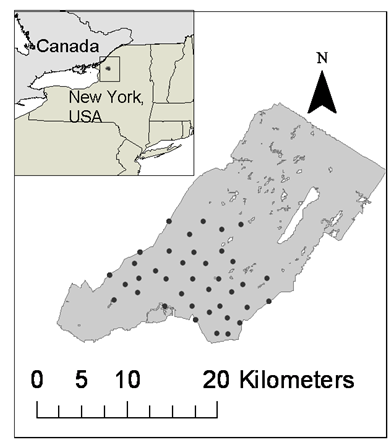
\includegraphics[height=2.5in,width=1.9in]{Ch3/figs/hairsnares.png}
\caption{Fort Drum Black bear study area and the 38 baited hair snare
  locations operated for 8 weeks during June and July, 2006.}
\label{fig.3.bears1}
\end{figure}

{\small
\begin{verbatim}
library("scrbook")
data("beardata")
trapmat<-beardata$trapmat
nind<-dim(beardata$bearArray)[1]
K<-dim(beardata$bearArray)[3]
ntraps<-dim(beardata$bearArray)[2]

M=175
nz<-M-nind
Yaug <- array(0, dim=c(M,ntraps,K))

Yaug[1:nind,,]<-beardata$bearArray
y<- apply(Yaug,c(1,3),sum) # summarize by ind x rep
y[y>1]<- 1                 # toss out multiple encounters
ytot<-apply(y,1,sum)       # total encounters out of K
\end{verbatim}
}

XXXX In these scripts change ytot to just y XXXXXXX

The raw data object, \mbox{\tt beardata\$bearArray} is a 3-dimensional
array $\mbox{\tt nind} \times \mbox{\tt ntraps} \times K$ of
individual encounter events (i.e., $y_{ijk} = 1$ if individual $i$ was
encountered in trap $j$ during occasion $k$, and 0 otherwise).  For
fitting model $M_{0}$ (or $M_{h}$, see below), it is sufficient to
reduce the data to individual encounter frequencies which we have
labeled \mbox{\tt ytot} above.  The {\bf BUGS} model file along with
commands to fit the model are as follows:

{\small
\begin{verbatim}
set.seed(2013)               # to obtain the same results each time
library("R2WinBUGS")
data0<-list(y=y,M=M,K=K)
params0<-list('psi','p','N')
zst=c(rep(1,nind),rbinom(M-nind, 1, .5))
inits =  function() {  list(z=zst, psi=runif(1), p=runif(1)) }

cat("
model {

psi~dunif(0, 1)
p~dunif(0,1)

for (i in 1:M){
   z[i]~dbern(psi)
   for(k in 1:K){
     tmp[i,k]<-p*z[i]
     y[i,k]~dbin(tmp[i,k],1)
      }
     }
N<-sum(z[1:M])
}
",file="modelM0.txt")

fit0 = bugs(data0, inits, params0, model.file="modelM0.txt",
       n.chains=3, n.iter=2000, n.burnin=1000, n.thin=1,
       debug=TRUE,working.directory=getwd())
\end{verbatim}
}
This produces the following posterior
 summary statistics:
{\small
\begin{verbatim}
> print(fit0,digits=2)
Inference for Bugs model at "modelM0.txt", fit using WinBUGS,
 3 chains, each with 2000 iterations (first 1000 discarded)
 n.sims = 3000 iterations saved
           mean    sd   2.5%    25%    50%    75%  97.5% Rhat n.eff
psi        0.29  0.04   0.22   0.26   0.29   0.31   0.36    1  3000
p          0.30  0.03   0.25   0.28   0.30   0.32   0.35    1  3000
N         49.94  1.99  47.00  48.00  50.00  51.00  54.00    1  3000
deviance 489.05 11.28 471.00 480.45 488.80 495.40 513.70    1  3000

[... some output deleted ...]
\end{verbatim}
}
{\bf WinBUGS} did well in choosing an MCMC algorithm for this model --
we have $\hat{R} = 1$ for each parameter, and an effective sample size
of 3000, equal to the total number of posterior samples\footnote{This is even a little
suspicious....}.
We see that the posterior mean of $N$ under this
model is $49.94$ and a 95\% posterior interval is $(48,54)$.  We
revisit these data later in the context of more complex models.

In order to obtain an estimate of density, $D$, we need an area to
associate with the estimate of $N$, and in Chapt.  \ref{chapt.intro}
we already went through a number of commonly used procedures to
conjure up such an area, including buffering the trap array by the
home range radius, often estimated by the mean maximum distance moved
(MMDM) \citep{parmenter_etal:2003}, $1/2$ MMDM \citep{dice:1938} or
directly from telemetry data \citep{wallace_etal:2003}
\begin{comment}
I HAVE SEEN 2 PAPERS CITING OTIS ET AL 1978 IN THIS CONTEXT
BUT I ONLY FOUND THE SECITON WHERE THEY SUGGEST USING INFORMATION ON ANIMAL HOME RANGE AS
OBTAIN FROM TRAPPING DATA; I GUESS THIS DICE GUY SAID TO USE THE HOME RANGE RADIUS
AND PEOPLE JUST TRY TO GET AT THIS WHICHEVER WAY THEY CAN; BE IT RECAPTURES OR OTHER HOME RANGE INFORMATION XXXXX).
\end{comment}
Typically, the trap array is defined by the convex hull around the
trap locations, and this is what we applied a buffer to. We computed
the buffer by using an estimate of the mean female home range radius
(2.19 km) estimated from telemetry studies \citep{bales_etal:2005}
instead of using an estimate based on our relatively more sparse
recapture data.  For the Fort Drum study, the convex hull has area
$157.135$ $km^2$, and the buffered convex hull has area $277.011$
$km^2$.  To create this we used functions contained in the {\bf R}
package \mbox{\tt rgeos} and created a utility function \mbox{\tt
  bcharea} which is in our {\bf R} package \mbox{\tt scrbook}. The
commands are as follows:
\begin{verbatim}
library("rgeos")

bcharea<-function(buff,traplocs){
p1<-Polygon(rbind(traplocs,traplocs[1,]))
p2<-Polygons(list(p1=p1),ID=1)
p3<-SpatialPolygons(list(p2=p2))
p1ch<-gConvexHull(p3)
 bp1<-(gBuffer(p1ch, width=buff))
 plot(bp1, col='gray')
 plot(p1ch, border='black', lwd=2, add=TRUE)
 gArea(bp1)
}

bcharea(2.19,traplocs=trapmat)
\end{verbatim}
The resulting buffered convex hull is shown in Fig. \ref{closed.fig.bch}.
\begin{figure}
\begin{center}
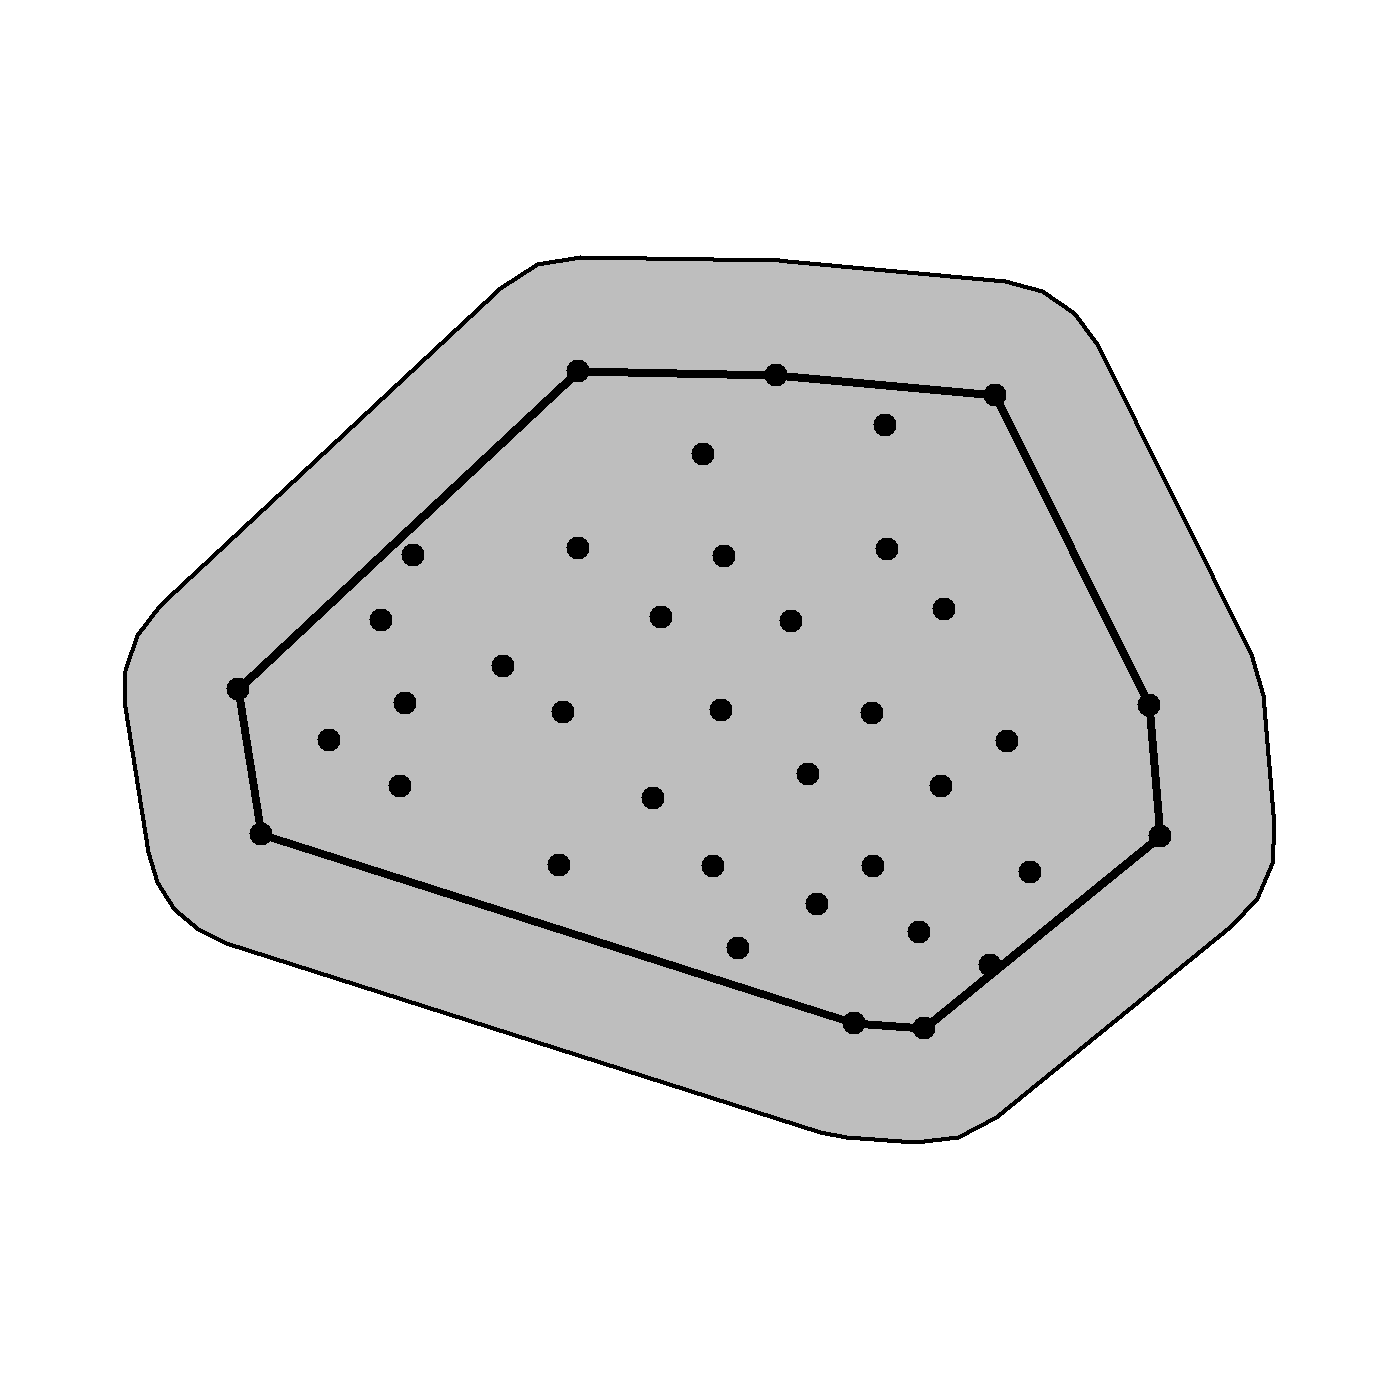
\includegraphics[height=3in,width=3in]{Ch3/figs/bufferedCH}
\end{center}
\caption{Convex hull of the bear hair snare array at Fort Drum, NY buffered by mean female
home range radius (2.19 km).}
\label{closed.fig.bch}
\end{figure}

To conjure up a
density estimate under model $M_0$, we compute the appropriate
posterior summary of the ratio of $N$ and the prescribed area ($277.011$ $km^2$):
{\small
\begin{verbatim}
> summary(fit0$sims.list$N/277.011)
   Min. 1st Qu.  Median    Mean 3rd Qu.    Max.
 0.1697  0.1733  0.1805  0.1803  0.1841  0.2130

> quantile(fit0$sims.list$N/277.011,c(0.025,0.975))
     2.5%     97.5%
0.1696684 0.1949381
\end{verbatim}
}
which yields a density estimate of about $0.18$ ind/km$^2$, and a $95\%$ Bayesian
confidence interval of $(0.170, 0.195)$.

In summary, we have an estimate of density if we have faith in our
stated value of the ``sample area''. Clearly though this is largely
subjective, and not something we can formally evaluate from the data.
How certain are we of this area? Can
we quantify our uncertainty about this quantity?
 More important, what exactly is
the meaning of this area and, in this context, how do we gauge bias
and/or variance of ``estimators'' of it? (i.e., what is it
estimating?).\footnote{Mention the delta approximation from
KARANTH AND NICHOLS (1998)?}
There is no theory to guide us in trying to answer these important questions.
XXX This is lame as shit XXXXX

\section{Temporally varying and behavioral effects}

The purpose of this chapter is mainly to emphasize the central
importance of the binomial model in capture-recapture and so we have
considered models for individual encounter frequencies - the number of
times individuals are captured out of $K$ samples.  Sometimes we can't
aggregate the encounter data for each individual, such as when
encounter probability varies over time among samples.  Time-varying
responses that are relevant in many capture-recapture studies are
``effort'' such as amount of search time, number of observers, or trap
nights, or when encounter probability varies over time or as a
function of date or season due to species behavior
\citep{kery_etal:2010}.  A common situation in many animal studies is
that in which there exists a ``behavioral response'' to trapping (even
if the animal is not physically trapped).
%For example, individuals might exhibit
%``trap happiness'' in response to baited traps. Conversely, individuals might learn
%to avoid traps (trap shyness) if the capture experience produces some negative
%stimulus.

Behavioral response is an important concept in animal studies
because individuals might learn to come to baited traps or avoid traps
due to trauma related to being encountered.  There are a number of
ways to parameterize a behavioral response to encounter. The
distinction between persistent and ephemeral was made by
\citet{yang_chao:2005} who considered a general behavioral response
model of the form:
\[
\mbox{logit}(p_{ik}) = \alpha_{0} + \alpha_{1}*y_{i,k-1} + \alpha_{2} x_{ik}
\]
where $x_{ik}$ is a covariate indicator variable of previous capture
(i.e., $x_{ik} = 1$ if captured in any previous period). Therefore,
encounter probability changes depending on whether an individual was
captured in the immediate previous period (ephemeral behavioral
response; \citep{yang_chao:2005}), described by the term
$\alpha_{1}*y_{i,k-1}$) or in any previous period (persistent behavioral
response).
%The former probably models a behavioral response due to
%individuals moving around their territory relatively slowly over time
%and the latter probably accommodates trap happiness due to baiting or
%shyness due to trauma.
Because spatial capture-recapture models allow us to include
trap-specific covariates, we can describe a 3rd type of behavioral
response -- a local behavioral response that is trap-specific
\citep{royle_etal:2011jwm}. In this local behavioral response, the
encounter probability is modified for an individual trap depending on
previous capture in that trap.

Models with temporal effects are easy to describe in the {\bf BUGS} language
and analyze and we provide a number of examples in
Chapt. \ref{chapt.covariates} and elsewhere.


\section{ Models with individual heterogeneity}
\label{closed.sec.modelmh}

Here we consider models with individual-specific encounter probability
parameters, say $p_{i}$, which we model according to some probability
distribution, $g(\theta)$. We denote this basic model assumption as
$p_{i} \sim g(\theta)$. This type of model is similar in concept to
extending a GLM to a GLMM but in the capture-recapture context $N$ is
unknown.  The basic class of models is often referred to as ``model
$M_h$'', but really this is a broad class of models, each being
distinguished by the specific distribution assumed for $p_{i}$.  There
are many different varieties of model $M_{h}$ including parametric and
various putatively non-parametric approaches
\citep{burnham_overton:1978, norris_pollock:1996, pledger:2000}. One
important practical matter is that estimates of $N$ can be extremely
sensitive to the choice of heterogeneity model
\citep{fienberg_etal:1999, dorazio_royle:2003, link:2003}. Indeed,
\citet{link:2003} showed that in some cases it's possible to find
models that yield precisely the same expected data, yet produce wildly
different estimates of $N$. In that sense, $N$ for most practical
purposes is not identifiable across classes of mixture models, and
this should be understood before fitting any such model. One solution
to this problem is to seek to model explicit factors that contribute
to heterogeneity, e.g., using individual covariate models (See
\ref{closed.sec.indcov} below). Indeed, spatial capture-recapture
models seek to do just that, by modeling heterogeneity due to the
spatial organization of individuals in relation to traps or other
encounter mechanism.  For additional background and applications of
model $M_{h}$ see \citet[][Chapt. 6]{royle_dorazio:2008} and
\citet[][Chapt. 6]{kery_schaub:2011}.

Model $M_{h}$ has important historical relevance to spatial
capture-recapture situations \citep{karanth:1995} because
investigators recognized that the juxtaposition of individuals with
the array of trap locations should yield heterogeneity in encounter
probability, and thus it became common to use some version of model $M_h$
in spatial trapping arrays to estimate $N$.  While this doesn't
resolve the problem of not knowing the area relevant to $N$, it does
yield an estimator that accommodates the heterogeneity in $p$ induced
by the spatial aspect of capture-recapture studies.

To see how this juxtaposition induces heterogeneity, we have to
understand the relevance of movement in capture-recapture models.
Imagine a quadrat that can be uniformly searched by a crew of
biologists for some species of reptile (see
\citet{royle_young:2008}).  Figure \ref{closed.fig.quadrat} shows a
sample quadrat searched repeatedly over a period of time. Further,
suppose that species exhibits some sense of spatial fidelity in the
form of a home range or territory, and individuals move about their
home range (home range centroids are given by the blue dots) in some
kind of random fashion.
%It is natural to think about it in terms of a
%movement process and sometimes that movement process can be modeled
%explicitly using hierarchical models \citep{royle_young:2008,
%  royle_etal:2011mee}.
Heuristically, we imagine that each individual in
the vicinity of the study area is liable to experience variable
exposure to encounter due to the overlap of its home range with the
sampled area - essentially the long-run proportion of times the
individual is within the sample plot boundaries, say $\phi$. We
might model the exposure of an individual to capture by supposing that
$z_{i} = 1$ if individual $i$ is available to be captured (i.e.,
within the survey plot) during any sample, and $0$ otherwise. Then,
$\Pr(z_{i}=1) = \phi$.  In the context of spatial studies, it is
natural that $\phi$ should depend on {\it where} an individual lives,
i.e., it should be individual-specific $\phi_{i}$
\citep{chandler_etal:2011}. This system describes, precisely, that of
``random temporary emigration'' \citep{kendall_etal:1997} where $\phi_{i}$
is the individual-specific probability of being ``available'' for
capture.

Conceptually, SCR models aim to deal with
this problem of variable exposure to sampling due to movement in the
proximity of the trapping array explicitly and formally with auxiliary
spatial information.  If individuals are detected with probability
$p_{0}$, {\it conditional} on $z_{i} = 1$, then the marginal
probability of detecting  individual $i$ is
\[
 p_{i} = p_{0}\phi_{i}
\]
so we see clearly that individual heterogeneity in encounter
probability is induced as a result of the juxtaposition of individuals
(i.e., their home ranges) with the sample apparatus and the movement
of individuals about their home range.

\begin{figure}
\begin{center}
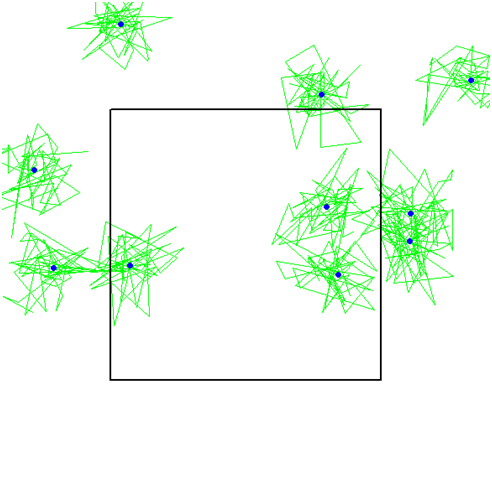
\includegraphics[height=3in]{Ch3/figs/quadrat}
\end{center}
\caption{A quadrat searched for lizards and the locations of each
  lizard over some period of time (simulated data).nice plot ! but, as usual, I would give more info. For instance, I would say something like ?Successive locations of 10 individual lizards over time are depicted by grey lines; black dots represent the individual activity centers.?}
\label{closed.fig.quadrat}
\end{figure}

We will work with a specific type of model $M_{h}$ here, that in which
we extend the basic binomial observation model of model $M_{0}$ so
that
\[
\mbox{logit}(p_{i}) = \mu + \eta_{i}
\]
where
\[
\eta_{i} \sim \mbox{Normal}(0, \sigma_{p}^2)
\]
We could as well write
\[
\mbox{logit}(p_{i}) \sim \mbox{Normal}(\mu,\sigma_{p}^2)
\]
This ``logit-normal mixture'' was analyzed by
\citet{coull_agresti:1999} and elsewhere. It is a natural extension of
the basic model with constant $p$, as a mixed GLMM, and similar models
occur throughout statistics. It is also natural to consider a beta
prior distribution for $p_{i}$ \citep{dorazio_royle:2003} and
so-called ``finite-mixture'' models are also popular
\citep{norris_pollock:1996, pledger:2000}. In the latter, individuals
are assumed to belong to a finite number of latent classes, each of
which has its own capture probability.


\subsection{Analysis of Model $M_h$}

If $N$ is known, it is worth taking note of the essential simplicity
of model $M_h$ as a binomial GLMM.  This is a type of model that is
widely applied throughout statistics using
standard methods of inference based either on integrated likelihood
\citep{laird_ware:1982, berger_etal:1999}, which we discuss in
Chapt. \ref{chapt.mle}, or standard Bayesian
methods. However, because $N$ is not known, inference is somewhat more
challenging. We address that here using Bayesian analysis based on
data augmentation (DA). Although we use data augmentation in the context of
Bayesian methods here, we note that
heterogeneity models formulated under DA are easily analyzed by
conventional likelihood methods as zero-inflated binomial mixtures
\citep{royle:2006} and more traditional analysis of model $M_h$ based on
integrated likelihood, without using data augmentation, has been
considered by \citet{coull_agresti:1999}, \citet{dorazio_royle:2003},
and others.

As with model $M_{0}$, we have the Bernoulli model for the
zero-inflation variables: $z_{i} \sim \mbox{Bern}(\psi)$ and the model
of the observations expressed conditional on these latent variables
$z_{i}$. For $z_{i}=1$, we have a binomial model with
individual-specific $p_{i}$:
\[
y_{i}|{z_{i} \! = \! 1} \sim \mbox{Bin}(K,p_{i})
\]
and otherwise $y_{i} |{ z_{i} \! = \! 0} \sim \delta(0)$. Further, we
prescribe a distribution for $p_{i}$. Here we assume
\[
\mathrm{logit}(p_{i}) \sim \mbox{Normal}(\mu,\sigma^2)
\]
For prior distributions we assume
$p_{0} = \mbox{logit}^{-1}(\mu) \sim
\mbox{Unif}(0,1)$ and, for the variance component
$\sigma \sim \mbox{Unif}(0,B)$ for some large $B$.
\begin{comment}
The basic {\bf BUGS} description for this model is given as follows:
{\small
\begin{verbatim}
model{

p0 ~ dunif(0,1)       # prior distributions
mup<- log(p0/(1-p0))
sigmap ~ dunif(0,10)
taup<- 1/(sigmap*sigmap)
psi~dunif(0,1)

for(i in 1:(nind+nz)){
  z[i]~dbern(psi)     # zero inflation variables
  lp[i] ~ dnorm(mup,taup) # individual effect
  logit(p[i])<-lp[i]
  mu[i]<-z[i]*p[i]
  y[i]~dbin(mu[i],K)  #  observation model
 }

N<-sum(z[1:(nind+nz)])  # N is a derived parameter
}
\end{verbatim}
}
\end{comment}
Another common default prior is to assume
$\tau = 1/\sigma^{2} \sim \mbox{Gamma}(.1,.1)$, although we usually
choose the $\sigma \sim \mbox{Unif}(0,B)$.



\subsection{Analysis of the Fort Drum data}
\label{closed.sec.Mhbear}
The logit-normal heterogeneity model was fitted to the bear data from
the Fort Drum study, and we used data augmentation to produce a data
set of $M=500$ individuals.  We ran the model using {\bf JAGS} with
the instructions given as follows:
{\small
\begin{verbatim}
[... get data as before ....]

set.seed(2013)

cat("
model{
p0 ~ dunif(0,1)       # prior distributions
mup<- log(p0/(1-p0))
sigmap ~ dunif(0,10)
taup<- 1/(sigmap*sigmap)
psi~dunif(0,1)

for(i in 1:(nind+nz)){
  z[i]~dbern(psi)     # zero inflation variables
  lp[i] ~ dnorm(mup,taup) # individual effect
  logit(p[i])<-lp[i]
  mu[i]<-z[i]*p[i]
  y[i]~dbin(mu[i],K)  #  observation model
 }

N<-sum(z[1:(nind+nz)])
}
",file="modelMh.txt")

data1<-list(y=ytot, nz=nz, nind=nind,K=K)
params1= c('p0','sigmap','psi','N')
inits =  function() {list(z=as.numeric(ytot>=1), psi=.6, p0=runif(1),
          sigmap=runif(1,.7,1.2),lp=rnorm(M,-2)) }

library("rjags")
jm<- jags.model("modelMh.txt", data=data1, inits=inits, n.chains=3,
                 n.adapt=10000)
jout<- coda.samples(jm, params1, n.iter=500000, thin=1)
\end{verbatim}
}
This produces the posterior distribution for $N$ shown
in Fig. \ref{closed.fig.bearMh}. Posterior summaries of parameters are
given as follows:
{\small
\begin{verbatim}
summary(jout)

[... output deleted ...]
Iterations = 500001:1e+06
Thinning interval = 1
Number of chains = 3
Sample size per chain = 5e+05

1. Empirical mean and standard deviation for each variable,
   plus standard error of the mean:

            Mean       SD  Naive SE Time-series SE
N      119.11050 57.85859 4.724e-02       1.285748
p0       0.07228  0.05545 4.527e-05       0.001064
psi      0.23928  0.11669 9.528e-05       0.002562
sigmap   2.08650  0.53532 4.371e-04       0.010903

xxxxxx
Could you explain this output a little more ? I later saw that you do
later on, but I would always explain new stuff where it first
appears. For instance, I had no clue what the naive SE meant ? Seems
to be the Monte Carlo error ?
xxxxxxxx

[... output deleted ... ]
\end{verbatim}
}

We used $M=500$ for this analysis and we
note that  while the posterior mass of $N$ is concentrated away from this
upper bound (Fig. \ref{closed.fig.bearMh}), the posterior has an
extremely long right tail, with some posterior values at the upper
bound $N=500$, suggesting that an even higher value of $M$ may be
called for.

To characterize the posterior distribution of density we produce the
relevant summaries of the posterior distribution of $N/277.11$ where,
recall, the buffered area of the convex hull is 277.11 $km^2$:
{\small
\begin{verbatim}
N<-c(jout[[1]][,"N"],jout[[2]][,"N"],jout[[3]][,"N"])
 summary(N/277.11)
   Min. 1st Qu.  Median    Mean 3rd Qu.    Max.
 0.1696  0.2959  0.3681  0.4298  0.4908  1.8040
> quantile(N/277.11,c(0.025,0.50,0.975))
     2.5%       50%     97.5%
0.2237379 0.3680849 1.0284724
\end{verbatim}
}
so the point estimate, characterized by the posterior mean, is around
$0.43$ bears per square km and a 95\% Bayesian credible interval is
$(0.224, 1.028)$.


The model runs effectively in {\bf WinBUGS} but sometimes with apparently
inefficient mixing for reasons that may be related to bad starting
values. In some cases this was resolved if we supplied starting values
for the $logit(p_{i})$ parameters and $\tau$. We provide a user-friendly {\bf R}
function \mbox{\tt modelMhBUGS} in the package \mbox{\tt scrbook} which will
fit the model using either {\bf JAGS} or {\bf WinBUGS} as specified by
the user.
In addition, for fun, we construct our own MCMC algorithm using a Metropolized
Gibbs sampler for model $M_{h}$ in Chapt. \ref{chapt.mcmc}, where we
also develop the MCMC  algorithms for spatial capture-recapture models.


\subsection{Comparison with MLE}

Because of the skewed posterior we see that the posterior mean
($N=119$) is considerably higher than the posterior median
($N=102$). Moreover, posterior summaries are estimated with a
relatively high error: The ``Time-series'' or Monte Carlo SE of around
1.2 (see secs.  for discussion of this quantity
\ref{glms.sec.convergence} \ref{mcmc.sec.mcmcsummary}) even despite
the high number of iterations we ran here (each of 3 chains based on
500000 iterations).  Further, it may be surprising that the posterior
mode does not compare well with the MLE which we presented in
sec. XXXX chapter 1 XXXXX which was XXXXXX.
To see this, we compute the posterior model by finding
the posterior value of $N$ with the highest mass, which is a
relatively easy proposition because $N$ is discrete.
 But we want to smooth out some of the Monte
Carlo error a bit so we used a smoothing spline to the posterior
frequencies of $N$ as follows (here we take only the first 80 values):
\begin{verbatim}
  tt<-table(jout[[1]][,"N"])[1:80]
  xg<-as.numeric(names(tt))
  plot(xg,tt)
  sp<- smooth.spline(xg,tt,df=9)
  sp$x[sp$y==max(sp$y)]
[1] 81
\end{verbatim}
The \mbox{\tt df} argument controls the degree of smoothing and we
find in this case that the modal value (i.e., 81) is not too sensitive
to the smoothing parameter but this should be checked in any specific
instance\footnote{we need to give examples of using \mbox{\tt
    density()} to obtain modes}.
To compare this with the MLE, we used
the {\bf R} code contained in Panel 6.1 from \citet{royle_dorazio:2008}.  The
MLE of $log(n_{0})$, the logarithm of the number of uncaptured
individuals, is $\widehat{log(n0)} = 3.86$ and therefore $\hat{N} =
exp(3.86)+47 = 94.47$ which is not at all consistent with the
mode in
Fig. \ref{closed.fig.bearMh}.
%\footnote{We note that the result is inconsistent with Gardner et
%  al. (2009) who reported an MLE of 104.1 ($density = 0.437
%  inds/km^2$) although we do not know the reason for this at the
%  present time.}
%To convert this to density we use the buffered area
%as computed above (255.3 $km^2$)\footnote{WRONG \#} and perform the
%required summary analysis on the posterior samples of $N$, which
%results in about $0.37$ individuals/$km^2$. The reader should carry
%out this analysis to confirm the estimates, and also obtain the $95\%$
%confidence interval.
\begin{comment}
We reflect for a moment on the whole idea of using
capture-recapture to estimate density. It seems pointless to argue about ``buffer width'' when
we can't even decide on an estimate of $N$! Maybe this reflects poorly
on the desire to have a point estimate of a quantity more than our
ability to provide
\end{comment}

{\bf Remarks:}
First of all the posterior for this model and data set is
very sensitive to prior distributions. While MLEs are invariant to
transformation of the parameters, the posterior distribution
definitely is {\it not} invariant. In the present case, the use of a
$\mbox{Unif}(0,1)$ prior for $p_{0} = \mbox{expit}(\mu)$ is somewhat
informative -- in particular, it is not at all ``flat'' on the scale
of $\mu$ -- and this affects the posterior.  We generally always
recommend use of a $\mbox{Unif}(0,1)$ prior for $\mbox{expit}(\mu)$ in such
models. That said, we were surprised at this result, and we
experimented with other prior configurations including putting a flat
prior on $\mu$ directly. That specific prior suggests the possibility
that the posterior distribution may be improper for that prior
specification. This kind of small sample instability has been widely
noted in model $M_h$ \citep{fienberg_etal:1999, dorazio_royle:2003},
as has extreme sensitivity to the specific form of model $M_{h}$ \citep{link:2003}.
In summary, while the mode is well-defined, the data set is relatively
sparse and hence inferences are poor and sensitive to model choice.

\begin{figure}
\centering
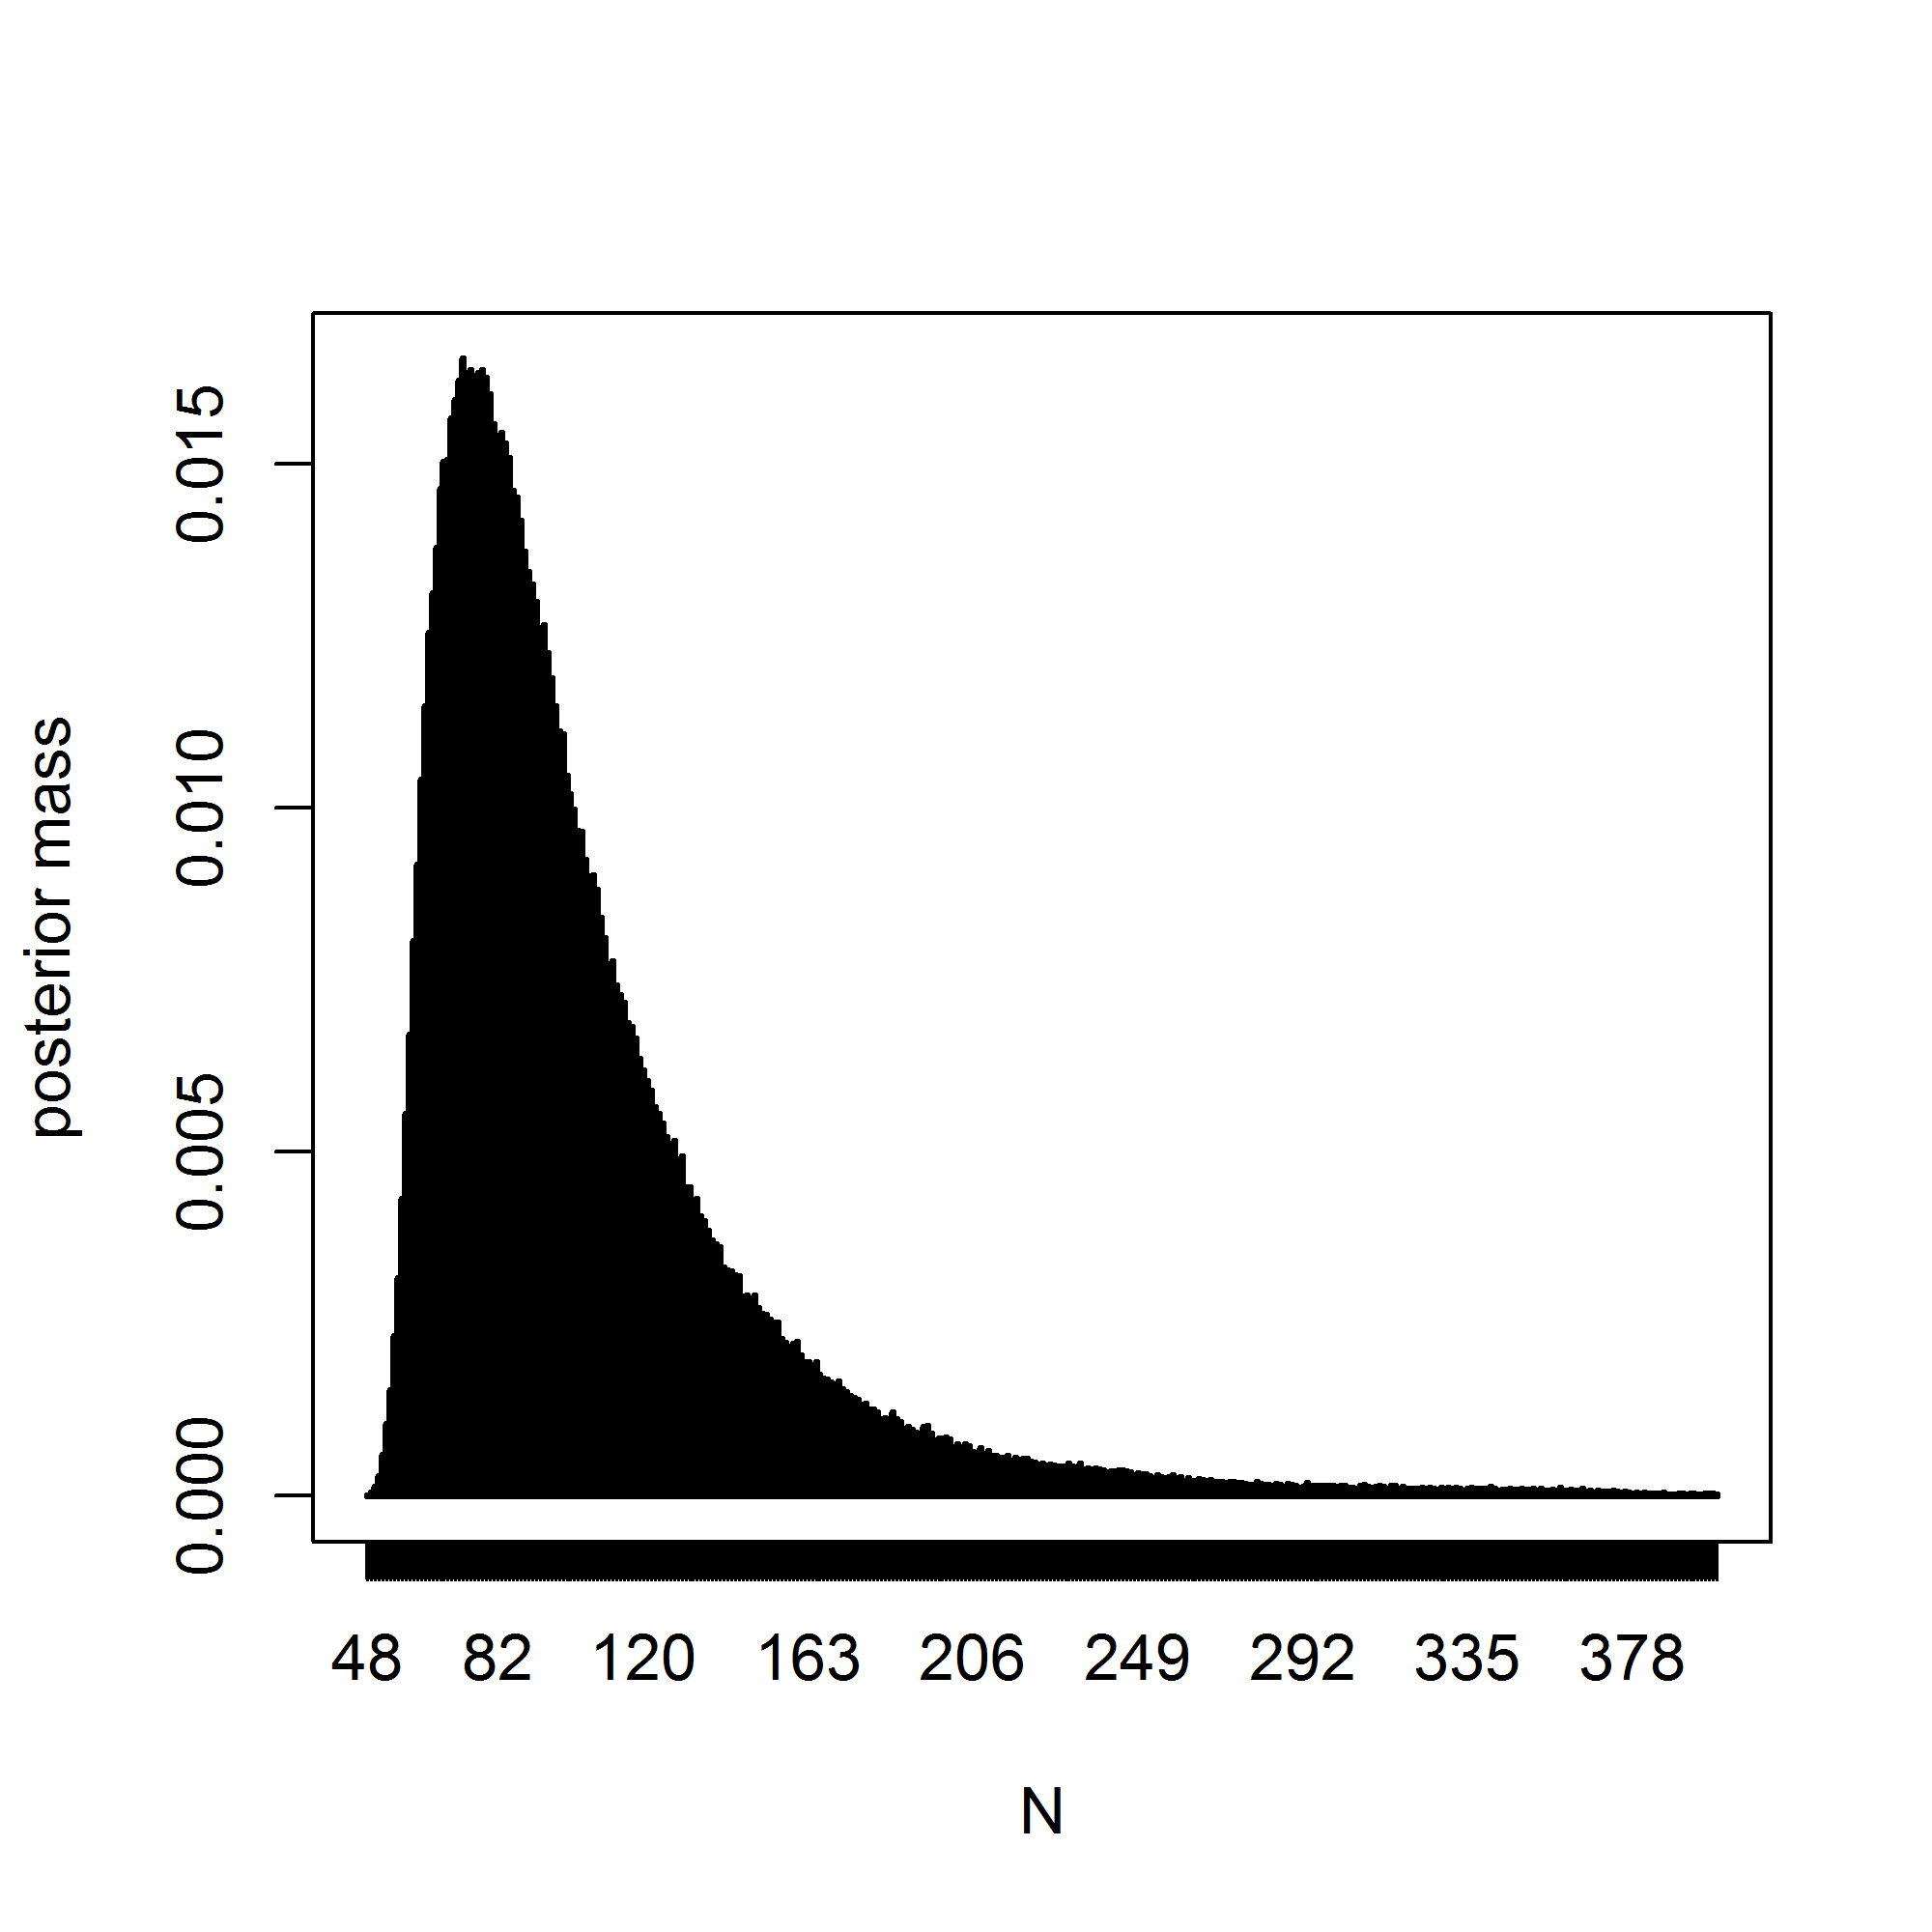
\includegraphics[height=4.5in,width=4.5in]{Ch3/figs/bear-modelMh-post}
\caption{Posterior of $N$ for Fort Drum bear study data under the
logit-normal version of model $M_h$.
}
\label{closed.fig.bearMh}
\end{figure}




\begin{comment}

To begin, we first collect all of our model components
which are as follows: $[y_{i}| p_{i},z_{i}]$,
$[p_{i}|\mu_{p},\sigma_{p}]$, and $[z_{i}|\psi]$
for {\it each} $i=1,2,\ldots,M$ and then prior distributions
$[\mu_{p}]$, $[\sigma_{p}]$ and $[\psi]$.
The joint posterior distribution of all unknown quantities in the model
is proportional to the joint distribution of all elements
$y_{i},p_{i},z_{i}$ and also the prior distributions of the prior parameters:
\[
\left\{ \prod_{i=1}^{M} [y_{i}|p_{i},z_{i}][p_{i}|\mu_{p},\sigma_{p}]
[z_{i}|\psi] \right\} [\mu_{p},\sigma_{p},\psi]
\]
For prior distributions, we assume that $\mu_{p},\sigma_{p}, \psi$ are
mutually independent and for $\mu_{p}$ and $\sigma_{p}$ we use
improper uniform priors, and $\psi \sim \mbox{Unif}(0,1)$.  Note that
the likelihood contribution for each individual, when conditioned on
$p_{i}$ and $z_{i}$, does not depend on $\psi$, $\mu_{p}$, or
$\sigma_{p}$.  As such, the full-conditionals for the structural
parameters $\psi$ only depends on the collection of data augmentation
variables $z_{i}$, and that for $\mu_{p}$ and $\sigma_{p}$ will only
depends on the collection of latent variables $p_{i}; i=1,2,\ldots,M$.
The full conditionals for all the unknowns are as follows:

{\bf (1)} For $p_{i}$:
\begin{eqnarray*}
[p_{i}|y_{i}, \mu_p, \sigma_{p},z_{i}=1] &\propto  &
[y_{i}|p_{i}][p_{i}|\mu_p,\sigma_{p}^{2}] \mbox{ if $z_{i}=1$ }  \\
                 &  &  [p_{i}|\mu_p,\sigma_{p}] \mbox{if $z_{i}=0$ }
\end{eqnarray*}

{\bf (2)} for $z_{i}$:
\[
z_{i} | \cdot \propto [y_{i}|z_{i}*p_{i}] \mbox{Bern}(z_{i}|\psi)
\]

{\bf (3)} For $\mu_{p}$:
\[
[\mu_{p} | \cdot ] \sim \prod_{i} [p_{i}| \cdot] *\mbox{const}
\]


{\bf (4)} For $\sigma_{p}$:
\[
[ \sigma_{p}|\cdot ] \sim\prod_{i}[p_{i}| \cdot ]*\mbox{const}
\]

{\bf (5)} For $\psi$:
\[
\psi|\cdot\sim \mbox{Beta}(1 + \sum z_{i}, 1 + M - \sum z_{i})
\]


We've  identified each of the full conditional
distributions in sufficient detail to apply the
Metropolis-Hastings algorithm. With the exception of $\psi$ which has
a convenient analytic solution -- it is a beta distribution which we
can easily sample directly. In truth, we could also sample $\mu_{p}$
and $\sigma_{p}^{2}$ directly with certain choices of prior
distributions. For example, if $\mu_{p} \sim \mbox{Normal}(0, 1000)$
then the full conditional for $\mu_{p}$ is also normal, etc..
We implement an MCMC algorithm for this model in the following block
of {\bf R} code.  The basic structure is: initialize the parameters
and create any required output or intermediate data holders, and then
begin the main MCMC loop which, in this case, generates 100000
samples.\footnote{This data grabbing function is not implemented yet}

{\small
\begin{verbatim}
## obtain the bear data by executing the previous data grabbing
## function

temp<-getdata()
M<-temp$M
K<-temp$K
ytot<-temp$ytot

###
### MCMC algorithm for Model Mh

out<-matrix(NA,nrow=100000,ncol=4)
dimnames(out)<-list(NULL,c("mu","sigma","psi","N"))
lp<- rnorm(M,-1,1)
p<-expit(lp)
mu<- -1
p0<-exp(mu)/(1+exp(mu))
sigma<- 1
psi<- .5
z<-rbinom(M,1,psi)
z[ytot>0]<-1

for(i in 1:100000){

### update the logit(p) parameters
lpc<- rnorm(M,lp,1)  # 0.5 is a tuning parameter
pc<-expit(lpc)
lik.curr<-log(dbinom(ytot,K,z*p)*dnorm(lp,mu,sigma))
lik.cand<-log(dbinom(ytot,K,z*pc)*dnorm(lpc,mu,sigma))
kp<- runif(M) < exp(lik.cand-lik.curr)
p[kp]<-pc[kp]
lp[kp]<-lpc[kp]

p0c<- rnorm(1,p0,.05)
if(p0c>0 & p0c<1){
muc<-log(p0c/(1-p0c))
lik.curr<-sum(dnorm(lp,mu,sigma,log=TRUE))
lik.cand<-sum(dnorm(lp,muc,sigma,log=TRUE))
if(runif(1)<exp(lik.cand-lik.curr)) {
 mu<-muc
 p0<-p0c
}
}

sigmac<-rnorm(1,sigma,.5)
if(sigmac>0){
lik.curr<-sum(dnorm(lp,mu,sigma,log=TRUE))
lik.cand<-sum(dnorm(lp,mu,sigmac,log=TRUE))
if(runif(1)<exp(lik.cand-lik.curr))
 sigma<-sigmac
}

### update the z[i] variables
zc<-  ifelse(z==1,0,1)  # candidate is 0 if current = 1, etc..
lik.curr<- dbinom(ytot,K,z*p)*dbinom(z,1,psi)
lik.cand<- dbinom(ytot,K,zc*p)*dbinom(zc,1,psi)
kp<- runif(M) <  (lik.cand/lik.curr)
z[kp]<- zc[kp]

psi<-rbeta(1, sum(z) + 1, M-sum(z) + 1)

out[i,]<- c(mu,sigma,psi,sum(z))
}
\end{verbatim}
}


{\bf Remarks}: (1) for parameters with bounded support, i.e.,
$\sigma_{p}$ and $p_{0}$, we are using a random walk candidate
generator but rejecting draws outside of the parameter space.  (2) We
mostly use Metropolis-Hastings except for the data augmentation
parameter $\psi$ which we sample directly from its full-conditional
distribution which is a beta distribution.  (3) Even the latent data
augmentation variables $z_{i}$ are updated using Metropolis-Hastings
although they too can be updated directly from their full-conditional.
\end{comment}


\begin{comment}

\subsection{Exercises related to model $M_h$}

\begin{itemize}
\item[(1)] Enclose the MCMC algorithm in an R function and provide
  arguments for some of the parameters of the function that a user
  might wish to modify.
\item[(2)] Execute the function and compare the results to those
  generated from WinBUGS in the previous section
\item[(3)] Note that the prior distribution for the ``mean'' parameter
  is given on $p_0=exp(\mu)/(1+exp(\mu))$.  Reformulate the algorithm
  with a flat prior on $\mu$ and see what happens. Contemplate this.
\item[(4)] Using Bayes rule, figure out the full conditional for
  $z_{i}$ so that you don't have to use MH for that one. It might be
  more efficient. Is it?
\item[(5)] Modify the MCMC algorithm so that the prior for $\mu_{p}$
  is an improper flat prior. i.e., $[\mu_{p}] \propto 1$. Describe the
  posterior distribution of $N$.
\end{itemize}

\end{comment}



\section{Individual Covariate Models: Toward Spatial Capture-Recapture}
\label{closed.sec.indcov}


A standard situation in capture-recapture models is when a
covariate which is thought
 to influence
encounter probability is measured for each individual.
As with other closed population models, we
begin with the basic binomial observation model:
\[
y_{i} \sim \mbox{Bin}(K, p_{i})
\]
and we assume also  a model for encounter probability according to:
\begin{equation}
 \mbox{logit}(p_{i}) = \alpha + \beta x_{i}
\label{closed.eq.ha}
\end{equation}
Classical examples of covariates influencing detection probability are
type of animal (juvenile/adult or male/female), a continuous covariate
such as body mass \citep[][ch. 6]{royle_dorazio:2008}, or a
discrete covariate such as group or cluster size. For example, in
models of aerial survey data, it is natural to model the detection
probability of a group as a function of the observation-level individual
covariate, ``group size'' \citep{royle:2008, royle:2009,
  langtimm_etal:2011}.

Such ``individual covariate models'' are similar in structure to model
$M_{h}$, except that the individual effects are {\it observed} for the
$n$ individuals that appear in the sample. These models are important
here because spatial capture-recapture models can be descrived precisely as a form of
individual covariate model, an idea that we will develop here and
elsewhere. Specifically, they are such models, but where the
individual covariate is a partially observed latent variable for
captured individuals. As such, it is a type of measurement error.
That is, unlike model $M_h$, we do have some direct information about the
latent variable, which comes from the spatial locations/distribution
of individual recaptures.

Traditionally, estimation of $N$ in individual covariate models is
achieved using methods based on ideas of unequal probability sampling
(i.e., Horvitz-Thompson estimation\footnote{For a  quick summary of
  the idea see:
  \url{http://en.wikipedia.org/wiki/Horvitz-Thompson_estimator}};
%see
\citet{huggins:1989},
\citet{alho:1990} and \citet{borchers_etal:2002}). An estimator of $N$ is
\[
\hat{N} = \sum_{i}^{n} \frac{1}{\tilde{p}_{i}}
\]
where $\tilde{p}_{i}$ is the probability that individual $i$ appeared
in the sample.  That is, $\tilde{p}_{i} = \Pr(y_{i}>0)$
where, in closed population capture-recapture models,
\[
\Pr(y_{i}>0) = (1- (1-p_{i})^K)
\]
where $p_{i}$ is a function of parameters $\alpha$ and $\beta$
according to Eq. \ref{closed.eq.ha}.  In practice, parameters are
estimated from the conditional-likelihood of the observed encounter
histories which is, for observation $y_{i}$,
\[
{\cal L}_{c}(\alpha, \beta | y_{i}) = \frac{ \mbox{Bin}(y_{i}|\alpha,\beta) } { \tilde{p}_{i}}.
\]

Here we take a formal model-based approach to Bayesian analysis of
such models based on the joint likelihood
using data augmentation \citep{royle:2009}. Classical
likelihood analysis of the so-called ``full likelihood'' is covered
 by \citet{borchers_etal:2002}.  For Bayesian analysis of
individual covariate models, because the individual covariate is
unobserved for the $N-n$ uncaptured individuals, we require a model to
describe variation among individuals, essentially allowing the sample
to be extrapolated to the population.  For our present purposes, we
consider a continuous covariate and we assume that it has a normal
distribution:
\[
x_{i} \sim \mbox{Normal}(\mu,\sigma^{2})
\]
Data augmentation can be applied directly to this class of models. In
particular, reformulation of the model under DA yields a basic
zero-inflated binomial model of the form:
\begin{eqnarray*}
z_{i} &\sim& \mbox{Bern}(\psi) \; \; \; i=1,2,\ldots,M\\
y_{i}|{z_{i}\! =\! 1} &\sim& \mbox{Bin}(K,p_{i}(x_{i})) \\
y_{i} |{ z_{i}\! =\! 0} &\sim& \delta(0)  \\
x_{i} & \sim & \mbox{Normal}(\mu,\sigma^{2})
\end{eqnarray*}
Fully spatial capture-recapture models use this
formulation with a latent covariate that is directly related to the
individual detection probability (see next section). As with the
previous models, implementation is trivial in the {\bf BUGS} language. The
{\bf BUGS} specification is very similar to that for model $M_h$, but we
require the distribution of the covariate to be specified, along with
priors for the parameters of that distribution.


\subsection{Example: Location of capture as a covariate.}

Here we consider a special type of individual covariate model that is
especially relevant to SCR.
If we had a regular grid of traps over some geographic region,
then we imagine that the average location of capture would be a decent
estimate (heuristically) of an individual's home range center.
Intuitively, some measure of typical distance from home range center to
traps for an individual should therefore be a reasonable  covariate to explain
heterogeneity in encounter probability, i.e., individuals with more
exposure to traps should have higher encounter probabilities and vice
versa.  A version of this idea was put forth by
\citet{boulanger_mclellan:2001} (see also \citet{ivan:2012}), but
using the Huggins-Alho estimator and with covariate ``distance to
edge'' of the trapping array. A limitation of this  approach is
that it does not provide a solution to the problem that the trap area
is fundamentally ill-defined, nor does it readily accommodate the
inherent and heterogeneous variation in this measured covariate.

We provide an example of this type of heuristically motivated
approach using a fully model-based individual covariate model
described above analyzed by data augmentation. We take a slightly
different approach than that adopted by
\citet{boulanger_mclellan:2001}. By analyzing the full likelihood and
placing a prior distribution on the individual covariate, we resolve
the problem of having an ill-defined area over which the population
size is distributed. After you read later chapters of this book, it
will be apparent that SCR models represent a formalization of this
heuristic procedure.

For our purposes here, we define $x_{i} = ||{\bf s}_{i} - {\bf
  x}_{0}||$ where ${\bf s}_{i}$ is the average encounter location of
individual $i$ and ${\bf x}_{0}$ is the centroid of the trap array.
Conceptually, individuals in the middle of the array should have a
higher probability of encounter and, as $x_{i}$ increases, $p_{i}$
should therefore decrease. We note that we have defined ${\bf s}_{i}$
in terms of a sample quantity - the observed mean - which is ad hoc
but consistent with existing applications in the literature.  For an
expansive, dense trapping grid we might expect the sample mean
encounter location to be a good estimate of home range center but,
clearly this is biased for individuals that live around the edge (or
off) the trapping array. Regardless, it should be good enough for our
present purposes of demonstrating this heuristically appealing
application of an individual covariate model. A key point is that
${\bf s}_{i}$ is missing for each individual that is not encountered
and so  $x_{i}$ is also missing. Therefore, it is a latent variable, or random
effect, and we need therefore to specify a probability distribution
for it.  As a measurement of distance we know it must be
positive-valued, and it seems sensible that an individual located
extremely far from the array of traps would not be captured.
Therefore,
 lets assume that $x_{i}$ is uniformly distributed from $0$ to some large number,
say $D_{max}$, beyond which it would be difficult to imagine an
individual being captured. For example, $D_{max}$ should be at a home
range diameter past the furthest trap from the center.  As such, we
use this distribution for the individual covariate ``distance from
center of the trap array''
\[
 x_{i} \sim \mbox{Unif}(0,D_{max})
\]
where $D_{max}$ is a specified constant, which we may choose to be
arbitrarily large.  In practice, people have
used distance from edge of the trap array but that is less easy to
make sense of.


\subsection{Fort Drum Bear Study}


We have to do a little bit of data processing to fit this individual
covariate model to the Fort Drum data.  We need to compute the
individual covariate ${\bf x}_{i}$ (distance from the centroid of the
trapping array) using the {\bf R} function \mbox{\tt spiderplot}
provided in \mbox{\tt scrbook}. This function also produces the keen
plot shown in Fig. \ref{closed.fig.spiderplot} which we call a
``spider plot''.  The {\bf R} commands for obtaining the individual
covariate ``distance from trap centroid'' and making the spider plot
are as follows:
\begin{verbatim}
library("scrbook")
data("beardata")
toad<- spiderplot(beardata$bearArray,beardata$trapmat)
xcent<-toad$xcent
\end{verbatim}
\begin{figure}
\centering
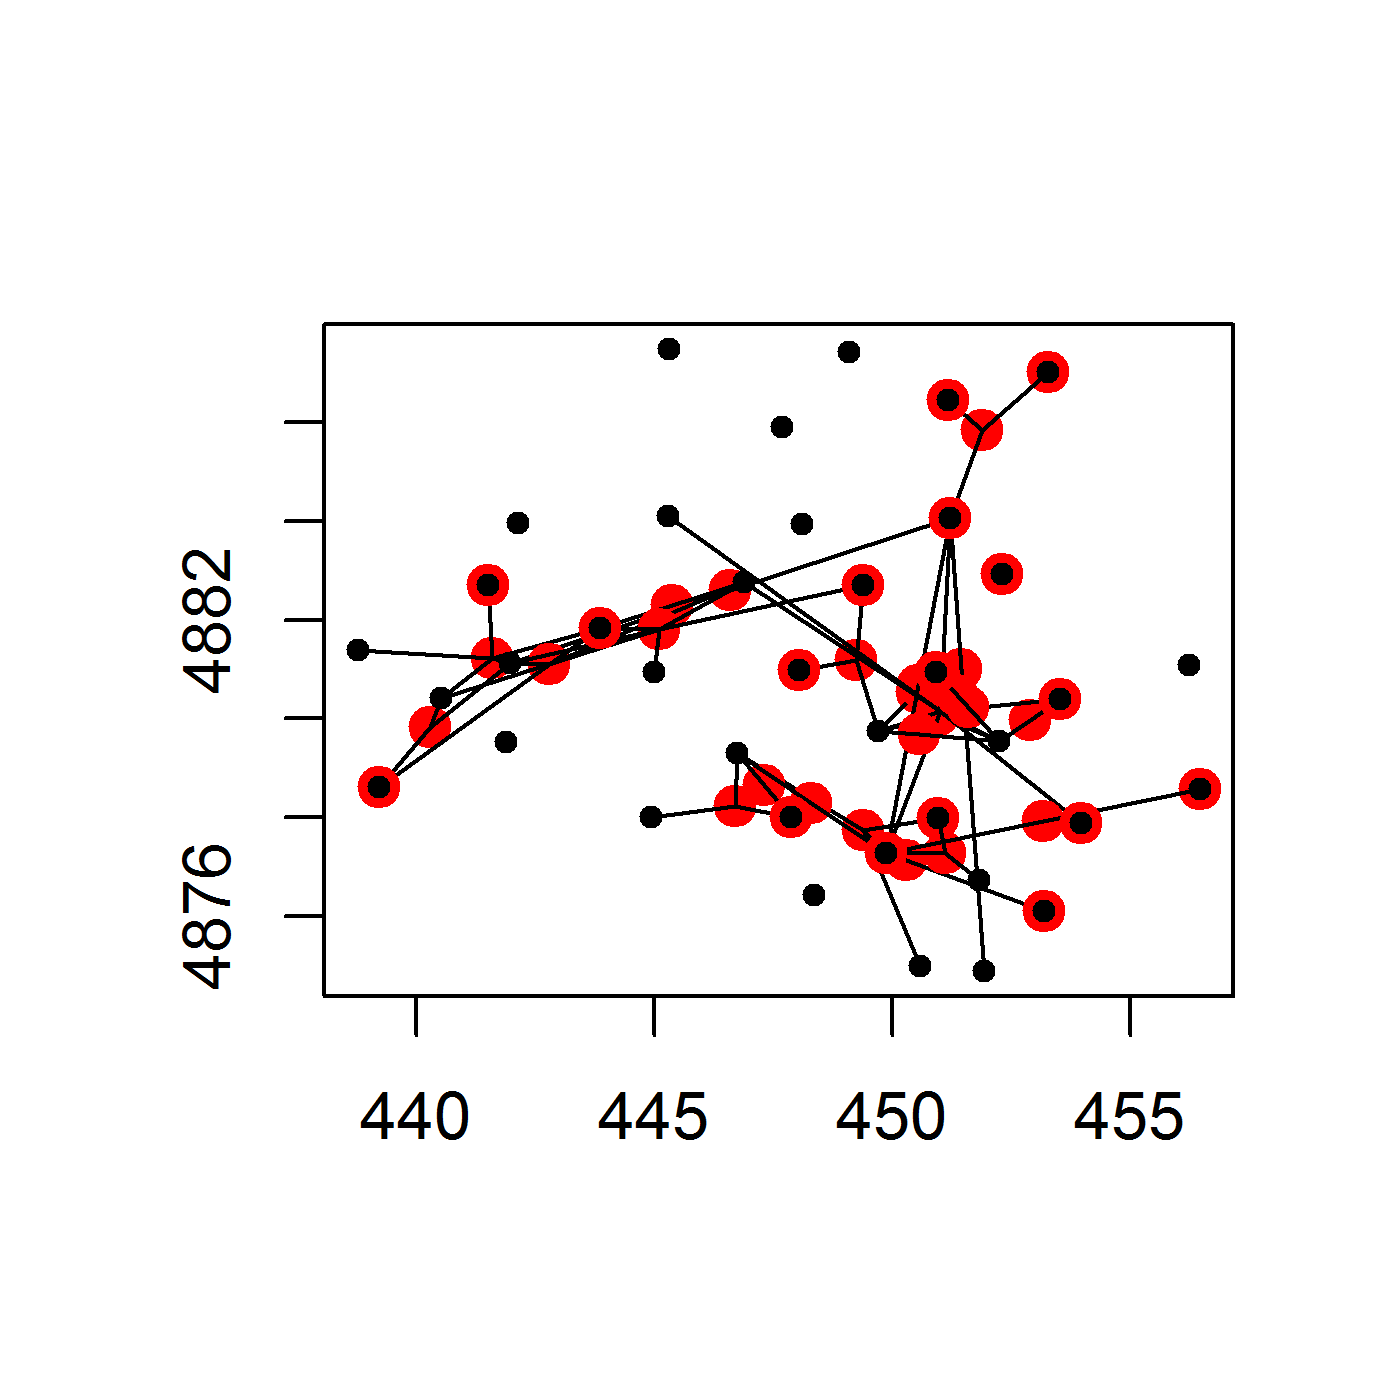
\includegraphics[height=3.5in,width=3.5in]{Ch3/figs/bear_spiderplot.png}
\caption{Spider plot of the Fort Drum study data.
The black dots represent the 47 trap locations with larger red dots
being the average capture location of each bear. i.e., its estimated home
range center. All traps in which a bear was captured are connected to
its estimated home range center with a line.
XXX note change one of the dots to an X or something XXXXX
}
\label{closed.fig.spiderplot}
\end{figure}

For the analysis of these data using the individual covariate
"distance from centroid" we used $x_{i} \sim \mbox{Unif}(0,D_{max})$
with $D_{max} = 11.5$ $km^2$, which is about the distance from the
array center to the furthest trap.  Once we pick $D_{max}$ then the
direct implication is that the population size parameter applies to
the area within 11.5 units of the trap centroid and thus we will find
that $N$ does, in fact, scale with our choice of $D_{max}$ to reflect
the changing area over which the $N$ individuals of the model reside.
The {\bf BUGS} model specification and {\bf R} commands to package the
data and fit the model are as follows:
{\small
\begin{verbatim}
cat("
model{
p0 ~ dunif(0,1)       # prior distributions
mup<- log(p0/(1-p0))
psi~dunif(0,1)
beta~dnorm(0,.01)

for(i in 1:(nind+nz)){
  xcent[i]~dunif(0,Dmax)
  z[i]~dbern(psi)     # DA variables
  lp[i] <- mup + beta*xcent[i] # individual effect
  logit(p[i])<-lp[i]
  mu[i]<-z[i]*p[i]
  y[i]~dbin(mu[i],K)  #  observation model
 }
N<-sum(z[1:(nind+nz)])
}
",file="modelMcov.txt")

data2<-list(y=ytot,nz=nz,nind=nind,K=K,xcent=xcent,Dmax=11.5)
params2<-list('p0','psi','N','beta')
inits =  function() {list(z=zst, psi=psi, p0=runif(1),beta=rnorm(1) ) }
fit2 =   bugs(data2, inits, params2, model.file="modelMcov.txt",working.directory=getwd(),
         debug=T, n.chains=3, n.iter=11000, n.burnin=1000, n.thin=1)
\end{verbatim}
}
This produces the following posterior summary statistics:
{\small
\begin{verbatim}
Inference for Bugs model at "modelMcov.txt", fit using WinBUGS,
 3 chains, each with 11000 iterations (first 1000 discarded)
 n.sims = 30000 iterations saved
           mean    sd   2.5%    25%    50%    75%  97.5% Rhat n.eff
p0         0.54  0.07   0.40   0.50   0.54   0.59   0.67    1  1100
psi        0.34  0.05   0.25   0.31   0.34   0.37   0.44    1  3500
N         58.92  5.49  50.00  55.00  58.00  62.00  71.00    1  1900
beta      -0.25  0.06  -0.36  -0.29  -0.25  -0.21  -0.12    1   780
deviance 459.51 13.21 435.80 450.20 458.80 467.90 487.40    1  2600
\end{verbatim}
}

It might be
perplexing that the estimated $N$ is much lower than obtained by model
$M_h$ but there is a good explanation for this, discussed
subsequently. That issue notwithstanding, it is worth pondering how
this model could be an improvement (conceptually or technically) over
some other model/estimator including $M_0$ and $M_h$ considered
previously. Well, for one, we have accounted formally for
heterogeneity due to spatial location of individuals relative to
exposure to the trap array, characterized by the centroid of the
array. Moreover, we have done so using a model that is based on an
explicit mechanism, as opposed to a phenomenological one such as Model
$M_h$. Moreover, importantly, using our new model, {\it the estimated N
  applies to an explicit area which is defined by our prescribed value
  of $D_{max}$}. That is, this area is a fixed component of the model and
the parameter $N$ therefore has explicit spatial context, as the number
of individuals with home range centers less than $D_{max}$ from the
centroid of the trap array. As such, the implied ``effective
area'' of the trap array for a given $D_{max}$ is a precisely defined
quantity -- it is that of a circle with with radius
$D_{max}$.


\subsection{Extension of the Model}

The model developed in the previous section
 is  not a very good model for one important reason:
Imposing a uniform prior distribution on $x$ implies that density is
{\it not constant} over space. In particular, this model implies that
it {\it decreases} as we move away from the centroid of the trap
array.  That is, $x_{i} \sim \mbox{Unif}(0,D_{max})$ implies constant
$N$ in each distance band from the centroid but obviously the {\it
  area} of each distance band is increasing.  This is one reason we
have a lower estimate of density than that obtained previously from
model $M_h$ (sec. \ref{closed.sec.Mhbear})
and also why, if we were to increase $D_{max}$, we would
see density continue to decrease.

Fortunately, the use of an individual covariate model is {\it not} restricted to
use of this specific distribution for the individual
covariate. Clearly, it is a bad choice and, therefore, we should think
about whether we can choose a better distribution for $D_{max}$ - one that
doesn't imply a decreasing density as distance from the centroid
increases.  Conceptually, what we want to do is impose a prior on
distance from the centroid, $x$, such that density is proportional to
the amount of area in each successive distance band as you move
farther away from the centroid.  In fact, theory exists
which tells us what the correct distribution of $x$ is:
$2x/D_{max}^2$. This can be derived by noting that $F(x) = \Pr(X<x) =
\pi*x*x/\pi*D_{max}^{2}$ . Then, $f(x) = dF/dx =
2*x/(D_{max}^{2})$. This is a sort of triangular distribution in
density
induced because the incremental area in each additional distance band
increases linearly with radius (i.e., distance from centroid). It is
sometimes comforting to verify things empirically:
{\small
\begin{verbatim}
 u<-runif(10000,-1,1)
 v<-runif(10000,-1,1)
 d<- sqrt(u*u+v*v)
 hist(d[d<1])
 hist(d[d<1],100)
 hist(d[d<1],100,probability=TRUE)
 abline(0,2)
\end{verbatim}
}

It would be useful if we could describe this distribution in {\bf
  BUGS} but there is not a built-in way to do this that we are aware
of.  One possibility is to use a discrete version of the pdf. We might
also be able to use what is referred to in {\bf WinBUGS} jargon as the
``zeros trick'' (see {\it Advanced BUGS tricks} in the manual)
although we haven't pursued this approach. Instead, we use a discrete
approximation of the density of $x$, and break $D_{max}$ into $L$
distance classes of width $\delta$, with probabilities proportional to
$2*x$. In particular, if we denote the cut-points by $xg_{1}=0,xg_{2},
\ldots, xg_{L+1}=D_{max}$ and the interval midpoints are $xm_{i} =
xg_{i+1}-\delta$ then the interval probabilities are $p_{i} =
2*xm_{i}*\delta/(D_{max}^{2})$, which we can compute once and then
pass them to {\bf WinBUGS} as data.

The {\bf R} commands for doing all of this (noting that we have
already loaded and processed the Fort Drum bear data) are given as
follows. In the model description the variable $x$ (observed distance
from centroid of the trap array) has been rounded so that the discrete
version of the $f(x)$ can be used as described previously. The new
variable labeled \mbox{\tt xround} is then the integer category label
in units of $\delta$ from 0. Thus, to convert back to distance in the
expression for $lp[i]$, \mbox{\tt xround[i]} has to be multiplied by
$\delta$. Here is the {\bf BUGS} model specification:
{\small
\begin{verbatim}
delta<-.2
xround<-xcent%/%delta  + 1
Dgrid<- seq(delta,Dmax,delta)
xprobs<- delta*(2*Dgrid/(Dmax*Dmax))
xprobs<-xprobs/sum(xprobs)

cat("
model{
p0 ~ dunif(0,1)       # prior distributions
mup<- log(p0/(1-p0))
psi~dunif(0,1)
beta~dnorm(0,.01)

for(i in 1:(nind+nz)){
  xround[i]~dcat(xprobs[])
  z[i]~dbern(psi)                     # zero inflation variables
  lp[i] <- mup + beta*xround[i]*delta # individual effect
  logit(p[i])<-lp[i]
  mu[i]<-z[i]*p[i]
  y[i]~dbin(mu[i],K)  #  observation model
 }

N<-sum(z[1:(nind+nz)])
}
",file="modelMcov.txt")
\end{verbatim}
}
To fit the model we do this - keeping in mind that the data objects
required below have been defined in previous analyses of this chapter:
{\small
\begin{verbatim}
data2<-list(y=ytot,nz=nz,nind=nind,K=K,xround=xround,xprobs=xprobs,delta=delta)
params2<-list('p0','psi','N','beta')
inits =  function() {list(z=z, psi=psi, p0=runif(1),beta=rnorm(1) ) }
fit = bugs(data2, inits, params2, model.file="modelMcov.txt",
          working.directory=getwd(), debug=FALSE, n.chains=3, n.iter=11000,
          n.burnin=1000, n.thin=2)
\end{verbatim}
}

This is a useful model because it induces a clear definition of area
in which the population of $N$ individuals reside. Under this model,
that area is defined by specification of $D_{max}$.
Further, the parameter $N$ of the model is, explicitly, the
population size that applies to the particular value of $D_{max}$ and,
as such, we will see that $N$ scales with our choice of $D_{max}$.
This might be disconcerting to some -- we can get whatever value of
$N$ we want by changing $D_{max}$!
Fortunately, we find empirically, that while $N$ seems
highly sensitive to the prescribed value of $D_{max}$, density seems to
be invariant to $D_{max}$ as long as it is chosen to be sufficiently
large. We fit the model for a random of values of $D_{max}$ from $D_{max}=12$ (restricting
values of $x$ to be in close proximity to
the trap array) on up to 20. The results are given in Table
\ref{closed.tab.Dmax}.

\begin{table}[htp]
\centering
\caption{Analysis of Fort Drum bear hair snare data using the
  individual covariate model, for different values of $D_{max}$, the upper
  limit of the uniform distribution of `distance from centroid of the
  trap array'. ``Density'' is the posterior mean of density and SD is
  the posterior standard deviation.}
\begin{tabular}{ccc}
\hline %\hline
 $D_{max}$ & Density & SD \\ \hline
  12& 0.230 & 0.038 \\
  15& 0.244 &0.041 \\
  17& 0.249 &0.044 \\
  18& 0.249 &0.043\\
  19& 0.250 &0.043\\
  20& 0.250 &0.044 \\
\hline
\end{tabular}
\label{closed.tab.Dmax}
\end{table}


We see that the posterior mean and SD of density (individuals per
square km) appear insensitive to choice of $D_{max}$ once we get away from the maximum observed value of about 11.5. The estimated
density of 0.25 per km$^2$ is actually quite a bit lower than we
reported using model $M_h$ for which no relevant ``area'' quantity is
explicit in the model.  Using MLEs of $N$ in conjunction with buffer
strips (see Table \ref{intro.tab.fdtests}) our estimates were in the
range of $0.32-0.43$ and see sec.  \ref{closed.sec.modelmh} above.  On
the other hand our estimate of $\hat{D} = 0.25$ here (based on the
posterior mean) is higher than that reported from model $M_0$ using
the buffered area (0.18). There is no basis really for comparing or
contrasting these various estimates and it would be a useful
philosophical exercise for the reader to discuss this matter. In
particular, application of models $M_0$ and $M_h$ are distinctly {\it
  not} spatially explicit models -- the area within which the
population resides is not defined under either model. There is
therefore no reason at all to think that the estimates produced under
either either closed population model, based on a buffered ``trap
area'', are justifiable by any theory. In fact, we would get exactly
the same estimate of $N$ no matter what we declare the area to be. On
the other hand, the individual covariate model explicitly describes a
distribution for ``distance from centroid'' that is a reasonable and
standard null model - it posits, in the absence of direct information,
that individual home range centers are randomly distributed in space
and that probability of detection depends on the distance between home
range center and the centroid of the trap array. Under this definition
of the system, we see that density is invariant to the choice of area,
which seems like a desirable feature.


\subsection{Invariance of density to $D_{max}$}

Under this individual covariate model, and also under models that we
consider in later chapters, a general property of the estimators is
that while $N$ increases with the prescribed trap area (equivalent to
$D_{max}$ in this case), we expect that density estimators should be
invariant to this area. In the model used above, we note that
$Area(D_{max}) = \pi*D_{max}^{2}$ and $E[N(D_{max})] =
\lambda*Area(D_{max})$ and thus $E[Density(D_{max})] = \lambda$, i.e.,
constant. This should be interpreted as the {\it prior}
density. Absent data, then realizations under the model will have
density $\lambda$ regardless of what $D_{max}$ is prescribed to be.
As we verified empirically above, the posterior density is also
invariant to $D_{max}$ as long as the implied area is large enough so
that the data no longer provide information about density (i.e., ``far
away'').

\subsection{Toward Fully Spatial Capture-recapture Models}

While the individual covariate model resolves two important problems
inherent in almost all capture-recapture studies (induced
heterogeneity and absence of a precise relationship between $N$ and
area), is not ideal for all purposes because it does not make full use
of the spatial information in the data set, i.e., the trap locations
and the locations of each individual encounter, so that we cannot use
this model to model trap-specific effects (e.g., trap effort or type).
Moreover, we developed this model for the average observed location
and equated it to home range center ${\bf s}_{i}$. Intuitively, taking
the average encounter location as an estimate of home range center
makes sense but more so when the trapping grid is dense and expansive
relative to typical home range sizes.  However, our approach also
ignored the variable precision with which each ${\bf s}_{i}$ is
estimated and also, as noted previously, estimates of ${\bf s}_{i}$
around the ``edge'' (however we define that) are biased because the
observations are truncated (we can only observe locations within the
trap array).

However, there is hope to extend this model in order to resolve
remaining deficiencies.  In the next chapter we provide a further
extension of this individual covariate model that definitively
resolves the ad hoc nature of the individual covariate approach we
took here. In that chapter we build a model in which ${\bf s}_{i}$ are
regarded as latent variables and the observation locations (i.e., trap
specific encounters) are linked to those latent variables with an
explicit model. We note that the model fitted previously could be
adapted easily to deal with ${\bf s}_{i}$ as a latent variable, simply
by adding a prior distribution for ${\bf s}_{i}$. The reader should
contemplate how to do this in {\bf BUGS}.


\section{Distance Sampling: A Primitive SCR Model}

Distance sampling is one of the most popular methods for estimating
animal abundance \citep{burnham_etal:1980, buckland_etal:2001,
  buckland_etal:2004book}. Unlike ordinary closed population models,
distance sampling provides explicit estimates of {\it density}, and
this is one of the main reasons it is so popular.  In terms of
methodological context, the distance sampling model is a special case
of a closed population model with an individual covariate. The
covariate in this case, $x_{i}$, is the distance between an
individual's location $u$ and the observation location or transect. In
fact, the model underlying distance sampling is precisely the same
model as that which applies to the individual-covariate models, except
that observations are made at only $K=1$ sampling occasion. Thus, in
that sense, distance sampling is a spatial capture-recapture model,
but without the ``recapture.''  This first and most basic spatial
capture-recapture model has been used routinely for decades and,
formally, it is a spatially-explicit model in the sense that it
describes, explicitly, the spatial organization of individual
locations (although this is not always stated explicitly) and, as a
result, somewhat general models of how individuals are distributed in
space can be specified \citep{hedley_etal:1999, royle_etal:2004,
  johnson_etal:2010, niemi_fernandez:2010, sillett_etal:2011}.

As before, the distance sampling model, under data augmentation,
includes a set of $M$ zero-inflation variables $z_{i}$ and the
binomial model expressed conditional on $z$ (binomial for $z=1$, and
fixed zeros for $z=0$).  In distance sampling we pay for having only a
single sample (i.e., $K=1$) by requiring constraints on the model of
detection probability, normally imposed as the assumption that
detection probability is $1.0$ when distance equals 0.  A standard
model is the ``half-normal'' model:
\[
\log(p_{i}) = \alpha_{1} x_{i}^{2}
\]
for $\alpha_{1} < 0$, where $x_i$ denotes the distance at which the $i$th
individual is detected relative to some reference location where
perfect detectability ($p=1$) is assumed. This function corresponds to
the ``half-normal'' detection function (i.e., with $\alpha_{1} =
1/\sigma^{2}$).  If $K>1$ then an intercept in this model is
identifiable and such models are usually called ``capture-recapture
distance sampling''\citep{alpizar_pollock:1996,borchers_etal:1998}.

As with previous examples, we require a distribution for the
individual covariate $x_{i}$. The customary choice is
\[
x_{i} \sim \mbox{Unif}(0,B)
\]
wherein $B>0$ is a known constant, being the upper limit of data
recording by the observer (i.e., the point count radius, or transect
half-width). In practice, this is sometimes asserted to be infinity,
but in such cases the distance data are usually truncated.
Specification of this distance sampling model in the {\bf BUGS} language is
shown in Panel \ref{closed.panel.distance} from \citet{royle_dorazio:2008}.


\begin{panel}[htp]
\centering
\rule[0.15in]{\textwidth}{.03in}
\begin{minipage}{5in}
\begin{verbatim}
alpha1~dunif(0,10)
psi~dunif(0,1)

for(i in 1:(nind+nz)){
   z[i]~dbern(psi)    # DA Variables
   x[i]~dunif(0,B)    # B=strip width
   p[i]<-exp(logp[i])   # DETECTION MODEL
   logp[i]<-   - alpha1*(x[i]*x[i])
   mu[i]<-z[i]*p[i]
   y[i]~dbern(mu[i])  # OBSERVATION MODEL
 }

N<-sum(z[1:(nind+nz)])
D<- N/striparea  # area of transects
\end{verbatim}
\end{minipage}
\rule[-0.15in]{\textwidth}{.03in}
\caption{Distance sampling model in {\bf BUGS}, using a half-normal
detection function.}
\label{closed.panel.distance}
\end{panel}

As with the individual covariate model in the previous section, the
distance sampling model can be equivalently specified by putting a
prior distribution on individual {\it location} instead of distance
between individual and observation point (or transect).  Thus we can
write the general distance sampling model as
\[
p_{i} = f(\alpha_{1},||{\bf u}_{i} - {\bf x}_0||)
\]
along with
\[
 {\bf u}_{i} \sim \mbox{Unif}({\cal S})
\]
where ${\bf x}_{0}$ is a fixed point (or line) and ${\bf u}_{i}$ is
the individual's location which is observable for $n$ individuals. In
practice it is easier to record distance instead of location.  Basic
math can be used to argue that if individuals have a uniform
distribution in space, then the distribution of Euclidean distance is
also uniform. In particular, if a transect of length $L$ is used and $x$
is distance to the transect then $F(x) = \Pr(X\le x) = L*x/L*B = x/B$ and
$f(x) = dF/dx = (1/B)$. For measurements of radial distance, see the
previous section.

In the context of our general characterization of SCR models
(Chapt. \ref{modeling.sec.characterization}),
we suggested that every SCR model can be described,
conceptually, by a hierarchical model of the form:
\[
 [y|u][u|s][s].
\]
Distance sampling ignores the part of the model pertaining to ${\bf
  s}$, and deals only with the model components for the observed
data  ${\bf u}$\footnote{Equivalently, we could also say that $[u]$ in
  the distance sampling model is $[u] = \int [u|{\bf s}][{\bf s}]
  d{\bf s}$}. Thus, we are left with a hierarchical model of the form
\[
[y|{\bf u}][{\bf u}].
\]
In contrast, as we will see in the next chapters, basic SCR models
(Chapt. \ref{chapt.scr0}) ignore ${\bf u}$ and condition on ${\bf s}$,
which is not observed:
\[
[y|{\bf s}][{\bf s}]
\]
Since $[{\bf u}]$ and $[{\bf s}]$ are both assumed to be uniformly
distributed, these are structurally equivalent models! The main
differences have to do with interpretation of model components and
whether or not the latent variables are observable (in distance
sampling they are).

So why bother with SCR models when distance sampling yields density
estimates and accounts for spatial heterogeneity in detection? For
one, imagine trying to collect distance sampling data on species such
as jaguars or tigers!  Clearly, distance sampling requires that one
can collect large quantities of distance data, which is not always
possible. For tigers, it is much easier, efficient, and safer to
employ camera traps or tracking plates and then apply SCR
models. Furthermore, as we will see in Chapts.
\ref{chapt.searchencounter} and \ref{chapt.scrds}, SCR models can use
distance data to estimate all the parameters of our big model
enchilada, allowing us to study distribution, movement, and
density. Thus, SCR models are much more general and versatile than
distance sampling models (which clearly are a special case), and can
accommodate data from virtually all animal survey designs.

\subsection{Example: Sonoran Desert Tortoise Study}

We illustrate the application of distance sampling models using data
on the Sonoran desert tortoise ({\it Gopherus agassizii}), shown in
Fig. \ref{closed.fig.tortoise}, collected along transects
in southern Arizona (see \citet{zylstra_etal:2010} for
details). The data are from 120 square transects having 4 250 m sides,
 although we ignore this detail in our analysis here and regard
them as 1 km transects, and we pooled the detection data from all
120 transects. The histogram of encounter distances from the 65
encounter individuals is
shown in Fig. \ref{closed.fig.tortoisehist}
\begin{figure}
\centering
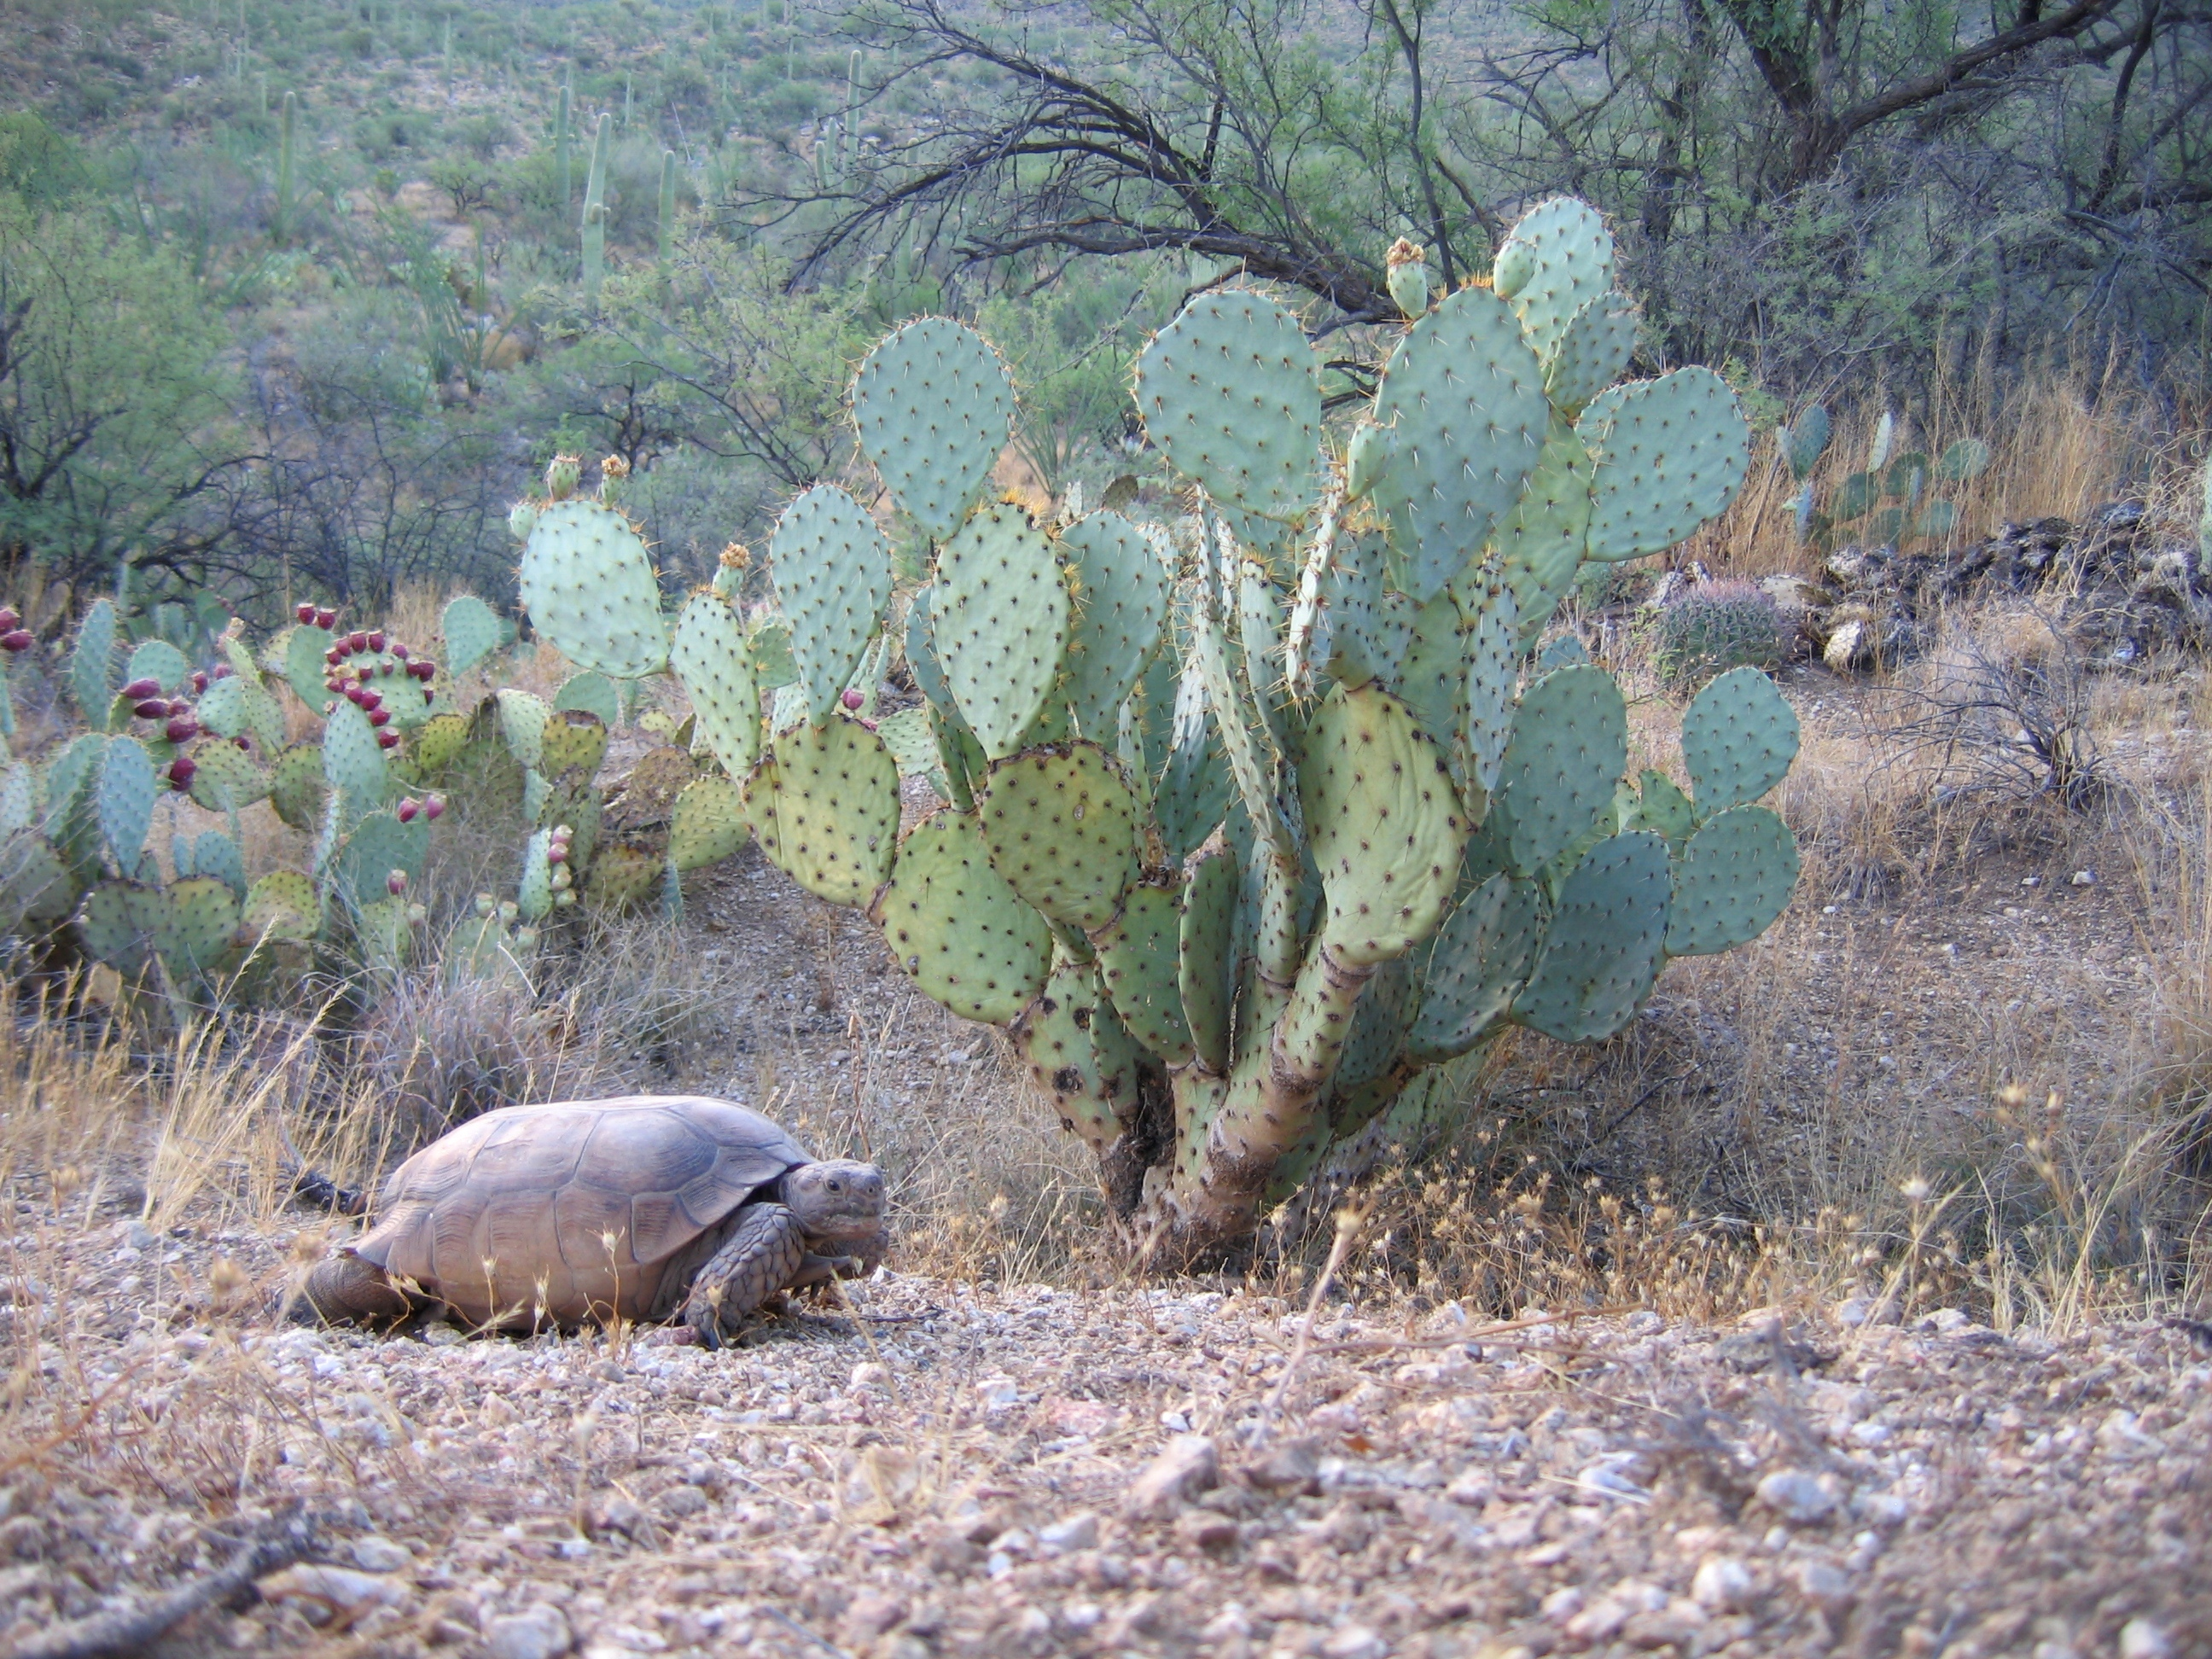
\includegraphics[height=3in,width=4in]{Ch3/figs/Erin_Zylstra_2.jpg}
\caption{Desert tortoise in its native habitat ({\it Photo credit: Erin
  Zylstra, Univ. of Arizona}.}
\label{closed.fig.tortoise}
\end{figure}

\begin{figure}
\centering
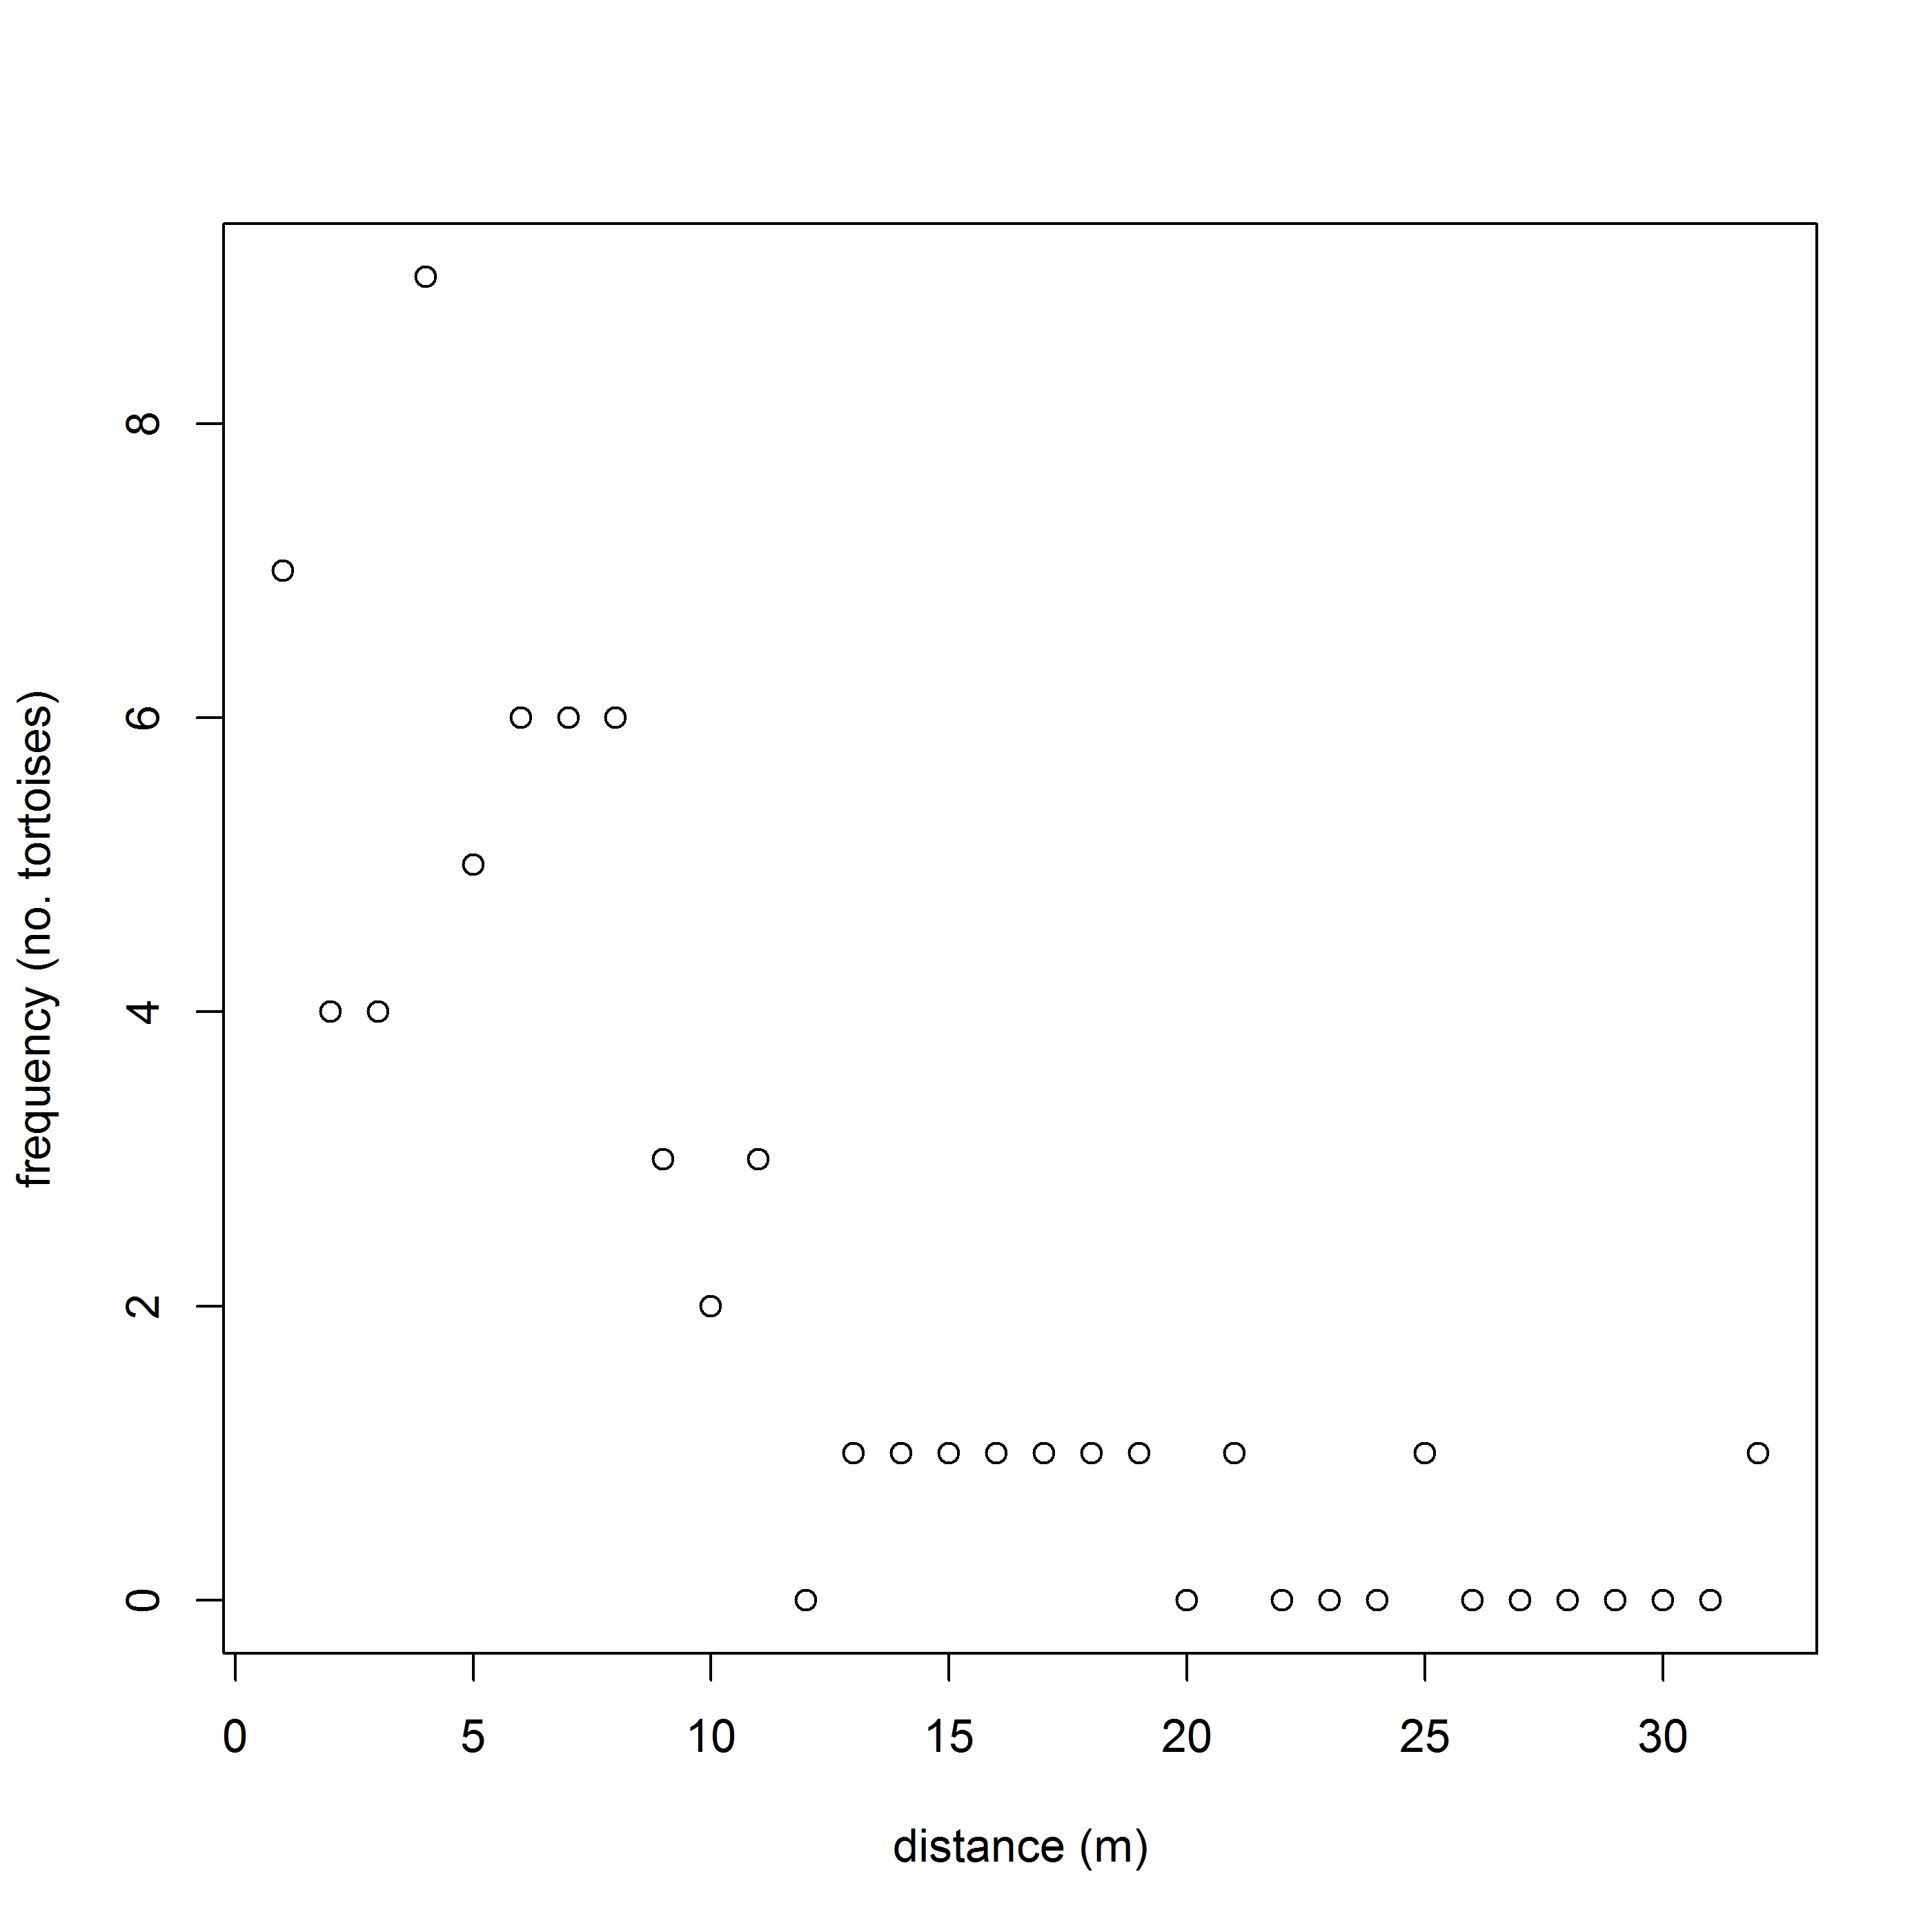
\includegraphics[height=3.35in,width=3.35in]{Ch3/figs/tortoise.png}
\caption{Histogram of Sonoran desert tortoise detections on 120 km of
transects.}
\label{closed.fig.tortoisehist}
\end{figure}

Commands
for reading in and organizing the data for analysis by {\bf WinBUGS}, followed by
writing the model to a text file, are given below. Note that the total sampled area of
the transects \mbox{\tt striparea} is input as data, and computed as:
$120$ (transects)
multiplied by the length ($1000$ m) and width ($B=40$ m), then
multiplied by 2, and then divided by $10000$ to make everything in units
of individuals {\it per} ha. The full script, provided with the
\mbox{\tt scrbook} {\bf R} package, we also give some commands for
analyzing the data using \mbox{\tt unmarked}
\citep{fiske_chandler:2011} using hierarchical distance sampling
models \citep{royle_etal:2004}.
{\small
\begin{verbatim}
data(toroise)
x<-tortoise[,"Dist"]
nind<-sum(!is.na(x))

y<-rep(1,nind)        # create encounter vector
nz<-700               # data augmentation
y<-c(y,rep(0,nz))     # add 0s to the encounter vector
x<-c(x,rep(NA,nz))    # pad distance vector with NA
z<-y                  # starting vals for data augmentation variables

cat("
model{
alpha1~dunif(0,10)
sigma<- sqrt(1/(2*alpha1))
psi~dunif(0,1)

for(i in 1:(nind+nz)){
   z[i]~dbern(psi)    # DA Variables
   x[i]~dunif(0,B)    # B=strip width
   p[i]<-exp(logp[i])   # DETECTION MODEL
   logp[i]<-   -alpha1*(x[i]*x[i])
   mu[i]<-z[i]*p[i]
   y[i]~dbern(mu[i])  # OBSERVATION MODEL
 }

N<-sum(z[1:(nind+nz)])
D<- N/striparea  # area of transects
}
",file="dsamp.txt")
\end{verbatim}
}

Next, we bundle the data,
provide initial values, indicate which parameters to monitor, and then
pass those things to {\bf WinBUGS}:
{\small
\begin{verbatim}
library("R2WinBUGS")

# density to be reported in units of ind/ha
data<-list(y=y,x=x,nz=nz,nind=nind,B=40,striparea=(120*1000*40*2/10000))
params<-list('alpha1','sigma','N','D','psi')
inits =  function() {list(z=z, psi=runif(1), alpha1=runif(1,0,.02) )}
fit = bugs(data, inits, params, model.file="dsamp.txt",working.directory=getwd(),
       debug=FALSE, n.chains=3, n.iter=3000, n.burnin=1000, n.thin=2)
\end{verbatim}
}
Posterior summaries are provided in the following summary
table. Estimated density (posterior mean) is $0.54$ individuals {\it
  per} ha and the estimated scale parameter of the distance function
(posterior mean) is $\sigma=9.12$ meters.  The Rhat statistics of
around $1.02$ suggest that slightly longer MCMC simulations might be
useful. The posterior mass of the data augmentation parameter $\psi$
is located away from the upper-bound $\psi=1$ and so the degree of
data augmentation appears sufficient.
{\small
\begin{verbatim}
> print(fit,digits=2)
Inference for Bugs model at "dsamp.txt", fit using WinBUGS,
 3 chains, each with 3000 iterations (first 1000 discarded), n.thin = 2
 n.sims = 3000 iterations saved
           mean    sd   2.5%    25%    50%    75%  97.5% Rhat n.eff
alpha1     0.01  0.00   0.00   0.01   0.01   0.01   0.01 1.02   130
sigma      9.12  0.77   7.77   8.57   9.07   9.62  10.77 1.02   130
N        516.67 54.71 415.00 478.00 516.00 552.00 632.00 1.02   100
D          0.54  0.06   0.43   0.50   0.54   0.57   0.66 1.02   100
psi        0.61  0.07   0.49   0.56   0.61   0.66   0.75 1.02    96

[.... some output deleted .... ]

\end{verbatim}
}




\begin{comment}
\subsection{Example: Muntjac deer survey from Nagarahole, India }


Here we fit distance sampling models to distance sampling data on the
muntjac deer (Muntiakus muntjak) collected in the year 2004 from
Nagarahole National Park in southern India
(Kumar et al. unpublished data). The muntjac is
a solitary species and distance measurements were made on 57 groups
that were largely singletons with 4 pairs of individuals.  Commands
for reading in and organizing the data for {\bf WinBUGS}, followed by
writing the model to a text file, are given below. Note that the total sampled area of
the transects is fed in as ``striparea'' which is $708$ (km of transect walked)
multiplied by the strip width ($B=120 = 0.12$ km) multiplied by 2.
{\small
\begin{verbatim}
library("R2WinBUGS")
data<- read.csv("Muntjac.csv")
hist(data[,3],30)
nind<-nrow(data)
y<-rep(1,nind)
nz<-400
y<-c(y,rep(0,nz))
x<-data[,3]
x<-c(x,rep(NA,nz))
z<-y

cat("
model{
beta~dunif(0,10)
psi~dunif(0,1)

for(i in 1:(nind+nz)){
   z[i]~dbern(psi)    # DA Variables
   x[i]~dunif(0,B)    # B=strip width
   p[i]<-exp(logp[i])   # DETECTION MODEL
   logp[i]<-   -beta*(x[i]*x[i])
   mu[i]<-z[i]*p[i]
   y[i]~dbern(mu[i])  # OBSERVATION MODEL
 }
N<-sum(z[1:(nind+nz)])
D<- N/striparea  # area of transects
}
",file="dsamp.txt")
\end{verbatim}
}
Next, we provide inits, indicate which parameters to monitor, and then
pass those things to {\bf WinBUGS}:
{\small
\begin{verbatim}
data<-list(y=y,x=x,nz=nz,nind=nind,B=120,striparea=(708*2*.120))
params<-list('beta','N','D','psi')
inits =  function() {list(z=z, psi=runif(1), beta=runif(1,0,.02) )}
fit = bugs(data, inits, params, model.file="dsamp.txt",working.directory=getwd(),
       debug=T, n.chains=3, n.iter=11000, n.burnin=1000, n.thin=2)
\end{verbatim}
}
Posterior summaries are provided in the following table. Estimated
density is pretty low, 1.1 individuals per sq. km.\footnote{ This is much
  lower than Samba's estimate produced from WinBUGS accounting for group
  size. Reason unknown. }
{\small
\begin{verbatim}
Inference for Bugs model at "dsamp.txt", fit using WinBUGS,
 3 chains, each with 11000 iterations (first 1000 discarded), n.thin = 2
 n.sims = 15000 iterations saved
           mean    sd   2.5%    25%    50%    75%  97.5% Rhat n.eff
beta       0.00  0.00   0.00   0.00   0.00   0.00   0.00    1  1100
N        185.73 26.53 138.00 167.00 184.00 203.00 242.00    1   570
D          1.09  0.16   0.81   0.98   1.08   1.20   1.42    1   570
psi        0.41  0.06   0.30   0.36   0.40   0.45   0.54    1   670
deviance 655.74 16.26 626.00 644.50 655.10 666.40 689.80    1  1300

xxxxxxx$Is the first line (beta) reasonable?$xxxxxxxxxx

[.... some output deleted .... ]
\end{verbatim}
}

\end{comment}























\section{Summary and Outlook}

Traditional closed population capture-recapture models are closely
related to binomial generalized linear models.  Indeed, the only real
distinction is that in capture-recapture models, the population size
parameter $N$ (corresponding also to the size of a hypothetical
``complete'' data set) is unknown.  This requires special
consideration in the analysis of capture-recapture models. The
classical approach to inference recognizes that the observations don't
have a standard binomial distribution but, rather, a truncated
binomial (from which which the so-called {\it conditional likelihood}
derives) since we only have encounter frequency data on observed
individuals. If instead we analyze the models using data augmentation,
the observations can be modeled using a zero-inflated binomial
distribution. In short, when we deal with the unknown-$N$ problem using
data augmentation then we are left with zero-inflated GLM and GLMMs
instead of ordinary GLM or GLMMs. The analysis of such zero-inflated
models is practically convenient, especially using the various
Bayesian analysis packages that use the {\bf BUGS} language.

Spatial capture-recapture models that we will consider in the rest of
the chapters of this book are closely related to what have been called
individual covariate models. Heuristically, spatial capture-recapture
models arise by defining individual covariates based on observed
locations of individuals -- we can think of using some function of
mean encounter location as an individual covariate. We did this in a
novel way, by using distance to the centroid of the trapping array as
a covariate. We analyzed the {\it full likelihood} using data
augmentation, and placed a prior distribution on the individual
covariate which was derived from an assumption that individual
locations are, a priori, uniformly distributed in space. This
assumption provides for invariance of the density estimator to the
choice of population size area (induced by maximum distance from the
centroid of the trap array). The model addressed some important problems in the
use of closed population models: it allows for heterogeneity in
encounter probability due to the spatial context of the problem and it
also provides a direct estimate of density because area is a feature
of the model (via the prior on the individual covariate). The model is
still not completely general because it does not make use of
the fully spatial encounter histories, which provide direct
information about the locations and density of individuals.  A
specific individual covariate model that is in widespread use is
classical distance sampling. The model underlying distance
sampling is precisely a special kind of SCR model - but one without
replicate samples. Understanding distance sampling and individual
covariate models more broadly provides a solid basis for understanding
and analyzing spatial capture-recapture models.

